\renewcommand{\thechapter}{4}
\chapter{Evaluation of NPS Return Flow to the River Using a Water Balance Model}
\label{chap:WaterBalanceModel}

\begin{linenumbers}
\section{Water Balance Model Applied to the LARV}
\label{sec:AppliedWaterModel}

\subsection*{Water Balance Model Equation.}
%\emph{II - Justify use of equation}\\
The purpose of the water balance model is to determine the volume of unaccounted for water in each reach.  We begin with a basic water balance model as describe in most hydrology texts --- \parencite{wanielista1997}.
\begin{equation}
	\textnormal{change in storage = inputs - outputs} \nonumber
\end{equation}

Adding the variables, both known and unknown, present in the LARV we have the following equation:
\begin{equation}
\label{eq:water1}
	\frac{\Delta S}{\Delta t} = Q_{in,US} + \sum Q_{in} + P + R + B - Q_{out,DS} - \sum Q_{out} - E - T - F 
\end{equation}
\begin{longtable}{rl}
%\begin{tabularx}{6in}{rX}
	Where: \\
	$\frac{\Delta S}{\Delta t}$ =&Stored volume change between time steps.\\
	$ Q_{in,US} $ = & Flow in the river entering the study reach at the upstream end.\\
	$ \sum Q_{in} $ = & Flow gained by the river from tributaries and other gauged sources.\\
	$ P $ = & Volume of water gained to the river due to precipitation falling directly on the river's surface.\\
	$ R $ = & Volume of water gained to the river due to precipitation runoff from adjacent land. \\
	$ B $ = & Volume of water gained to the river due to subsurface flow. \\
	$ Q_{out,DS} $ = & Flow in the river leaving the study reach at the downstream end.\\
	$ \sum Q_{out} $ & Flow lost from the river to canals and other gauged sinks.\\
	$ E $ = & Volume of water lost from the river due to direct evaporation from the water's surface.\\
	$ T $ = & Volume of water lost from the river due to plant transpiration.\\
	$ F $ = & Volume of water lost from the river due to infiltration into the subsurface flow.\\
%\end{tabularx}
\end{longtable}

If we combine the terms that are unknown or unmeasured, we arrive at the following equation:
\begin{equation}\label{eq:water01}
	\frac{\Delta S}{\Delta t} = Q_{in,US} + \sum Q_{in} + P - Q_{out,DS} - \sum Q_{out} - E + Q_{NPS}
\end{equation}
\begin{tabularx}{6in}{rX}
	Where: \\
	\Qnps = & The sum of gains from non-point sources and losses to non-point sinks $ \left( Q_{NPS} = R + B - T - F + Q_{U,in} - Q_{U,out}\right) $.\\ 
\end{tabularx}\\

%\emph{III - define $Q_U$ constituents}\\
There is no reasonable method for differentiating the components of \Qnps, therefore the abbreviation NPS in this thesis refers to both non-point sources and non-point sinks.   \Qnps includes the non-point source gains from groundwater sources($ B $), non-point source losses to groundwater sinks {}$ F $), transpiration losses from plants in the river channel ($ T $), and gains from precipitation runoff from adjacent land ($ R $).  Additionally, this term includes ungauged flows leaving and entering the river.  Ungauged gains to the river ($ Q_{U,in} $) are suspected to be primarily in the form of irrigation drainage from adjacent farmland.  Other sources could be due to errors in underestimating flows entering the river or overestimating flows leaving the river.  Ungauged losses from the river ($ Q_{U,out} $) are suspected to be primarily in the form of minor or unauthorized withdrawals from the river channel.  Of the ungauged flows, irrigation drainage from adjacent farmlands is assumed to be the largest contributor.

The two groundwater components of \Qnps are suspected of being the largest components of \Qnps.  Water transfer between the aquifer and river happens continually whereas $ Q_{U,in} $, $ Q_{U,out} $, $ R $, and $ T $ are not continuous.  $ Q_{U,in} $ and $ Q_{U,out} $ only occur periodically when individuals actively withdraw from the river or allow irrigation runoff to return to the river.  $ R $ only occurs during rain events.  Within the LARV, most rainwater is captured in irrigation canals.  Only precipitation falling in the riparian zone is likely to reach the river.  $ T $ only occurs during growing season.  This value is also only considering the transpiration happening within the river channel and does not include the riparian zone.  Any losses due to transpiration in the riparian zone are first considered river losses to the aquifer ($ F $).


Re-arranging equation \eqref{eq:water01} to solve for the unknown values produces equation \ref{water02}.  Due to the nearly identical method of calculating flow ($ Q $) and it's associated error and uncertainty, these terms were associated with each other.  Likewise, the precipitation ($ P $) and evaporation ($ E $) terms were associated with each other.
\begin{equation}\
Q_{UNPS} = \left( Q_{out,DS} + \sum Q_{out} - Q_{in,US} - \sum Q_{in} \right) - \frac{\Delta S}{\Delta t} - \left( P + E \right)\\ \label{water02}
\end{equation}

A time step of one day was established for all models calculated in this thesis.  Most of the data from agencies is readily available in average daily format.  While most of the data could also be obtained in hourly or quarter-hourly format, it was assumed that the additional information would not improve model accuracy.

\clearpage{}
\section{Stochastic and Deterministic Models}
\label{sec:StochAndDetermModels}

Deterministic and stochastic models are used in both the unaccounted for water and mass balance models.  Deterministic models are fully determined by the input parameters or variables.  Randomness of any kind is not included.  Stochastic models extend deterministic models by including one or more random parameters.  Given the same input parameter values, a stochastic model will produce different results with each iteration.

There are many recognized methods for solving stochastic models.  Solutions to these models are not definite and the term "solve" must be taken loosely.  Any individual solution from a stochastic model is one of a potentially infinite number of possible solutions.  The Monte Carlo (MC) simulation technique was used to obtain solutions for all stochastic models in this thesis.  The MC technique is conceptually simple.  The stochastic model is repetitively solved in a series of iterations.  The combined solutions from all iterations are used to define the solution statistics of the model.  

The number of iterations performed is determined by calculating and analyzing a set of identifier statistic(s) after each run.  Identifier statistic(s) are those that the modeler has determined to be of value in determining when to terminate the model.  These statistics are monitored to identify when the change in the statistic has reached a predetermined threshold.  It was determined that for the sake of simplicity, all of the models calculated in this thesis would use the same number of iterations.  The USR mass balance model is the most complex model as it has the largest number of input variables and uncertainty terms.  The identifier statistics used were the mean, variance, and skewness which are the first, second, and third moments of the probability density.  These were calculated for each iteration.  The threshold between the observed iteration and the previous iteration was fixed at 0.1\%.  The identifier statistics reached the threshold in the following order: mean, variance, and skewness.  Skewness reached its break point shortly before the 500th iteration.  A judgment call was made to increase the factor of safety.  Therefore, the number of stochastic model iterations was fixed at 5,000.  The fourth moment, kurtosis, was also calculated and analyzed for each iteration.  It was found to be too sensitive as it did not consistently stay within the accepted cutoff threshold of 0.1\%.  It is assumed that this sensitivity is due to the existence of a significant number of outliers that cause the distribution of results to be non-normal.

\section{Error and Uncertainty.}
\label{sec:ErrorAndUncertainty}

Any problem that measures variable natural processes must account for parameter and model uncertainties \parencite{vicens1975}.  Parameter uncertainty is derived from measurement error, spatial variability, and temporal variability \parencite{herschy2002}.  Measurement error is the difference between the true and measured values.  Most of this error type is due to instrument measurement inaccuracies due to either error inherent in the instrument or from errors in calibration or measurement.  Measurement errors inherent to the instrument are uncorrectable and cannot be accounted for within the model.  Errors due to calibration or measurement deviations are only correctable at the time of measurement or calibration and cannot be accounted for within the model.

Spatial variability is the difference in the true value at different points when measured at the same time.  Data collected at a single given point in space may not be representative of the area it is assumed to represent due to spatial variability.  This can manifest itself even with very small distances between measurements.  Temporal variability is the difference in the true value at the same point, but at different times.  Data collected at a one time may not be representative of the time frame it is assumed to represent due to temporal variability \parencite{Gates1996}.  Again, this can be manifested even over small time differences.  Due to instrument error, the spatiotemporal variability of the measured object, and the inability to know the true value of the measurement, reported parameter values should be treated as random variables \parencite{haan1989,haan2002}.

Almost all of the data was obtained from outside agencies and was not collected by the research team.  These agencies have data uncertainty ranges that account for all parameter uncertainties.  These uncertainties are expressed in accordance with the ISO Guide to Expression of Uncertainty in Measurement (GUM) \parencite{gum2008}.  While the GUM classifies uncertainty as either "Type A" or "Type B", the all of the data included in this thesis has uncertainty evaluations described as "Type B".  Type B evaluations usually use standard deviations and assumed probability distributions obtained from scientific judgment, available information, and possible variability of a measurement.

The data originators have provided uncertainty ranges which include instrument measurement random error and uncertainties due to temporal variations of the measured location.  The root mean square method is used to estimate the uncertainty related to measurement of water quantity and water quality values \parencite{harmel2007, gum2008}.  \textcite{harmel2007} describe this measurement uncertainty as the “probably error range”, and quantify upper and lower uncertainty boundaries for measured data points as the following when attempting to specify an expected range of expected values.

\begin{align}
	\sigma^2 = \left( \frac{O_i-UO_{i}(l)}{3.9} \right)^2  &  \phantom{xxxxxxxx} or  & 	\sigma^2 = \left( \frac{UO_{i}(u)-O_i}{3.9} \right)^2 \label{eq:uncertainty1}
\end{align}

\begin{tabular}{r p{5in}}
	Where:\\
	$ \sigma^2 $ = & variance about measured data value $ O_i $.\\
	$ O_i $ = & measured value.\\
	$ UO_i $ = & upper $ (u) $ and lower $ (l) $ uncertainty boundaries.\\
	$ 3.9 $ = & number of standard deviations accounting for $ >99.99 $\% of a normal probability distribution\\
\end{tabular}\\

The data collected for this thesis is assumed to represent the mean of a normal distribution of possible values.  The upper and lower bounds of the distributions are given as either a percent or value deviation from the mean.  Equation \ref{eq:uncertainty1} is re-written from the definition found in \textcite{harmel2007} to that found in equation \ref{eq:uncertainty2}.

\begin{align}
	\sigma^2 = \left( \frac{\mu - (\mu - \mu p)}{3.9} \right)^2  &  \phantom{wordsssssss} or \phantom{s}  & 	\sigma^2 = \left( \frac{(\mu + \mu p) - \mu}{3.9} \right)^2 \label{eq:uncertainty2}
\end{align}

\begin{tabular}{r p{5in}}
	Where:\\
	$ \mu $ = & the reported value (assumed to be the mean).\\
	$ p $ = & the reported percent deviation from $ \mu $.\\
\end{tabular}\\

Both of these equations in \ref{eq:uncertainty2} simplify to equation \ref{eq:uncertainty3}.  The standard deviation is shown as the calculated result due to the requirements of the modeling software.

\begin{equation}
\sigma = \frac{\mu p}{3.9}
\label{eq:uncertainty3}
\end{equation}

When the upper and lower bounds are defined as a fixed value deviation from the reported value, then equation \ref{eq:uncertainty1} becomes:

\begin{align}
	\sigma^2 = \left( \frac{\mu - (\mu - v)}{3.9} \right)^2  &  \phantom{wordsssssss} or \phantom{s}  & 	\sigma^2 = \left( \frac{(\mu + v) - \mu}{3.9} \right)^2 \label{eq:uncertainty4}
\end{align}

\begin{tabular}{r p{5in}}
	Where:\\
	$ v $ = & the reported value deviation from $ \mu $.\\
\end{tabular}\\

In this case, both equations in \ref{eq:uncertainty4} simplify to:

\begin{equation}
\sigma = \frac{v}{3.9}
\label{eq:uncertainty5}
\end{equation}

The difference between a model's calculated or estimated value and the reported value is called a residual.  The distribution of residuals is the model uncertainty.  These distributions are uni-variate and do not have predefined shapes.  There are a variety of statistical and graphical tools available to analyze unknown residual distributions to determine a best fit parametric distribution.  The two graphical tools used in this thesis to analyze distributions are the histogram and the kernel density estimate.

Non-parametric distribution models are used as an aid for analyzing uni-variate data sets.  Specifically, kernel density estimates (KDE) are used in conjunction with histograms to assist in visual analysis of the data.  Figure \ref{fig:ExampleDistAnalysis} is an example of a random sample of one of the input data sets used in this thesis.  The curve is the KDE.  The short vertical lines between the histogram and the x-axis, called a rug, depict the data values.  This figure adequately displays the resulting differences between histograms and KDE.  KDEs can more accurately depict data groupings that are lost in histogram bins.  The histogram leads us to believe that the data has a strong tendency to be near zero, wile the KDE shows that the majority of the data is between 0-20.  Histograms can more accurately depict extremes or cut-off values.  In the figure, there are no values less than zero.  The histogram clearly shows this while the KDE shows that there are values less than zero.  Both histograms and KDE are used throughout this thesis to assist in the description of distributions.  A rug is also presented with the histogram whenever the quantity of data allows for adequate data presentation.  A rug is not included when the data set is too large to allow for discreet identification of data values.

\begin{figure}[htbp]
\begin{center}
	\includegraphics[width=6in]{"Figures/Example KDE"}
	\caption[Example kernel density estimate.]{Example kernel density estimate.  The data is a random sample of an input variable used in this thesis.  The curve depicts the kernel density estimate.  The short vertical lines between the histogram and the x-axis, called a rug, depict the data values.}
	\label{fig:ExampleDistAnalysis}
\end{center}
\end{figure}

Determining which parametric distribution best fits the uni-variate residual distribution requires the use of both the graphical and statistical tools.  For each residual distribution, probable parametric distributions types were chosen for testing against the residual distribution.  For each of these parametric distribution types, a best fit was generated using the maximum likely-hood estimator  (MLE) method.  These MLE results were then analyzed using Kolmogorov-Smirnov (K-S),  Cramer-von Mises (CvM), and Anderson-Darling (A-D) goodness-of-fit tests to determine which distribution type best fit the uni-variate residual distribution.  All three tests are non-parametric tests of continious uni-variate probability distributions.  The K-S and CvM tests calculate the difference between the empirical cumulative density function (ECDF) of the test data and the cumulative density function (CDF) of the tested reference distribution.  The K-S and CvM tests use different algorithms to perform the calculation.  Each of the goodness-of-fit tests has their own strength and weaknesses and as such, graphical tools are used to confirm or refute the statistical test results \parencite{delignette2014, venables2002, DAgostino1986}.

\clearpage{}
\section{River Storage Change}
\label{sec:RiverStorageChange}

%\emph{0 - define the equation and variables}
River reach estimated stored water volume changes $( \frac{\Delta S}{\Delta t} ) $ from equation \ref{eq:water1} are the sum of the river segment stored water volume changes for each reach (Equation \ref{eq:storage1}).  The storage change for each segment is calculated independent of adjacent segments.

\begin{equation}
	\label{eq:storage1}
	\frac{\Delta S}{\Delta t} = \sum \frac{\Delta S_i}{\Delta t}
\end{equation}

\begin{tabular}{rl}
Where:\\
$\Delta S$ = & Water storage change in the river reach.\\
$\Delta S_i$ = & Water storage change in river segment $ i $.\\
$ \Delta t $ = & Model time step = 1 day. \\
\end{tabular}\\

%\emph{II - define calculation of storage change}\\
River reach volume changes are calculated between two consecutive time steps.  Reach volume changes are calculated as the sum of the volume changes within the segments that compose the reach.  River segment volume change between time steps is calculated as shown in equation \ref{eq:volumesimple}.
\begin{equation}
	\frac{\Delta S_i}{\Delta t}=L_i \cdot \frac{\Delta A_i}{\Delta t}
	\label{eq:volumesimple}
\end{equation}
\begin{tabular}{r l}
	Where:&\\
	$\frac{\Delta S_i}{\Delta t}$ & = Segment storage change.\\
	$L_i$ & = Segment length.\\
	$\frac{\Delta A_i}{\Delta t} $ &= Segment cross-section area change.\\
\end{tabular}\\

Figure \ref{fig:segment model} shows the difference between a simplified example of a natural channel and the modeled channel.  Although the river is variable in width and depth along its entire lengths, it  is modeled as a trapezoidal prism with a constant length and with a cross-section that does not vary with respect to location.  It was reasoned that this simplistic model would best approximate the average channel shape along the entire reach.  The channel water surface elevation is assumed to be constant through each segment.  This assumption is not true in nature, but we are not concerned with the water surface elevation, but with the flow depth.  We are assuming that the flow depth remains relatively constant through a river segment.  This assumes that all gains and losses to the river are accounted for either through flow gains and losses, evaporation, precipitation, or unaccounted for gains and losses as shown in equation \ref{eq:water1}.

\begin{figure}[htbp]
	\begin{center}
		\includegraphics[width=6.5in]{"Figures/LineDiagram/PlanProfile"}
		\caption[River Segment Model.]{River Segment Model.}
		\label{fig:segment model}
	\end{center}
\end{figure}

Segment lengths, as reported in Table \ref{tab:SegmentLength}, are sufficiently short such that any surges due to irrigation canal gates changes, precipitation events, or other events pass through the segment in less than a day.  The total travel time is approximately 2-3 days and 1-2 days in the USR and DSR, respectively, based on USGS reported average stream velocity measurements taken in conjunction with stream gauge calibrations.  River segment length ($L_i$) was measured to the nearest \SI{0.1}{\kilo\meter} using publicly available satellite imagery, USGS hydrography data, and geographical information system (GIS) software.  River segment length was calculated as the length of the thalweg between the segment endpoints.  When the USGS thalweg did not follow along the river channel as shown in the satellite imagery, a new thalweg was drawn.  Rough validation of these measurements was performed in the field by comparing the GIS calculated length of adjacent roadways to the actual driven distance as reported by a vehicle odometer.  River lengths are assumed to be constant throughout the study time frame.  Individual and combined variations in the channel path along a river segment were assumed to be negligible.

\begin{table}[htbp]
	\centering
	\caption[River Segment Lengths.]{River Segment Lengths.}
	\label{tab:SegmentLength}
	\begin{tabular}{cccc}
		\toprule
		Study                & River   & \multicolumn{2}{c}{Segment Length} \\ \cmidrule(r{.5em}l){3-4}
		Reach                & Segment & km               & mi              \\
		\toprule
		\multirow{5}{*}{USR} & A       & 12.5             & 7.8             \\
		& B       & 3.9              & 2.4             \\
		& C       & 30.7             & 19.1            \\
		& D       & 37.8             & 23.5            \\
		& E       & 14.3             & 8.9             \\
		\midrule
		\multirow{2}{*}{DSR} & F       & 37.6             & 23.4            \\
		& G       & 24.9             & 15.5           \\
		\bottomrule
	\end{tabular}
\end{table}

River segment cross-sectional area change $\left( \frac{\Delta A_i}{\Delta t} \right) $ calculation is based on the trapezoidal area that approximates the difference between the cross-sectional area at two different flow depths as depicted in Figures \ref{fig:XSArea}, \ref{fig:XSTrapezoid} and in equation \ref{eq:XSArea}.  While the cross sectional area difference isn't exactly a trapezoid, the difference for small differences in gauge height is insignificant.  

\begin{figure}[htbp]
\begin{center}
	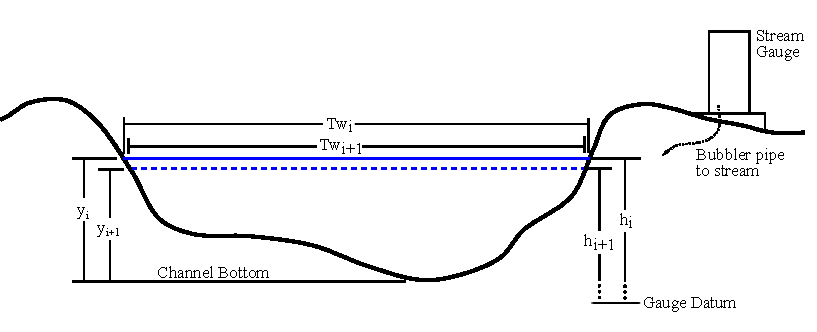
\includegraphics[width=6in]{Figures/LineDiagram/XSection}
	\caption[Average river segment cross-section area change.]{Average river segment cross-section area change.}
	\label{fig:XSArea}
\end{center}
\end{figure}

\begin{figure}
	\begin{center}
		\includegraphics[width=6.5in]{"Figures/LineDiagram/Trapezoid"}
		\caption[River cross-section area change diagram.]{River cross-section area change diagram.}
		\label{fig:XSTrapezoid}
	\end{center}
\end{figure}

\begin{align}
	\frac{\Delta A_i}{\Delta t}= & \overline{Tw}\cdot \Delta y \nonumber \\
	\frac{\Delta A_i}{\Delta t} = & \frac{Tw_t + Tw_{t-1}}{2} \cdot \left( y_{t-1} - y_t \right) \label{eq:XSArea}
\end{align}
\begin{tabular}{rl}
	Where: & \\
	$_t$ = & Current time step. \\
	$_{t-1}$ = & Previous time step. \\
	$\frac{\Delta A_i}{\Delta t}$ = & Cross-section area change at river section $ i $ between time steps.\\
	$\overline{Tw}$ = & Average river top width.\\
	$\Delta y$ = & Change in flow depth from the previous time step. \\
	$Tw$ = & River top width. \\
	$y$ = & River flow depth. \\
\end{tabular}\\

Figure \ref{fig:XSArea} shows a simplified river cross section at a stream gauge location.  As previously discussed, stream gauges do not hold the channel bottom as their datum.  They have an arbitrarily fixed datum that does not move unless reset by the gauge owner.  The difference between the stream gauge datum and the channel bottom is corrected using a constant correction factor calculated from the river survey.  The gauge datum does not have a known marker where the elevation could be directly measured.  Instead, the surveyed water surface elevation was recorded at the gauge location on both sides of the channel.  The flow depth value was calculated by finding the difference between the surveyed average water surface elevation and the surveyed channel bottom elevation.  The flow depth was then compared to the stream gauge height reported for the same date and time as when the water surface elevation was surveyed.  The difference between the reported value and the average of the surveyed values was taken as the correction factor for the gauge.  This procedure was repeated for each gauge.

Flow depth values as reported by the USGS and CDWR are measured values with an associated probability range as calculated in equation \ref{eq:uncertainty3}.  The uncertainties are applied as shown in equation \ref{eq:herror1}.  A correction factor ($ C_{i} $) is applied to each reported gauge depth to correct for the difference between the gauge datum and the channel bottom as measured during the channel cross-section survey.  Two separate uncertainties are applied.  $ \varepsilon_{h1} $ is the uncertainty distribution as described by the gauge owner.  This uncertainty is reported by both the USGS and CDWR as being normally distributed with extreme values at \SI{0.01}[$\pm$]{\foot} (\SI{0.003}[$ \pm $]{\meter}) \parencite{USGSPL89}.  The second uncertainty term, $ \varepsilon_{h2} $, is the result of personal observation of the river channel along its entire length.  This term describes the variability in flow depth.  It was observed that the channel depth did not vary greatly along most of its length.  There were particular areas where there were deeper pools, but these areas were noted to be more prone to ponding during low flow.  It is assumed that the average effective flow depth only varies within a normal distribution with limits of \SI{0.076}[$ \pm $]{\meter} (\SI{0.25}[$ \pm $]{\foot}).  There is the possibility that $\varepsilon_{h1}$ could cause the storage change between the time steps to change from a storage gain to a storage loss, or vise versa.  This is acceptable as it is within the measurement limits of the instruments.  Once $h+\varepsilon_{h1}$ has been calculated for the two successive time steps, the relationship between the two time steps is fixed.  If the river segment flow depth rises between time steps after this calculation, then that relationship must continue throughout the rest of the volume change calculation.  To facilitate this, it is assumed that $\varepsilon_{h2}$ does not vary significantly within the study time frame and does not vary within a realization.  The Arkansas River channel is sufficiently stable between consecutive days that this assumption is valid.  A new $\varepsilon_{h2}$ is drawn for each realization and remains constant for all time steps within the study time frame.

\begin{equation}
	y_{i,t}=h_{i,t}+C_{i}+\varepsilon_{h1}+\varepsilon_{h2}
	\label{eq:herror1}
\end{equation}
\begin{tabular}{rl}
	Where: & \\
	$y_{i,t}$  & = Section $ i $ modeled average daily flow depth at time $ t $.\\
	$h_{i,t}$  & = Section $ i $ reported average daily river gauge height at time $ t $.\\
	$ C_{i} $ & = Section $ i $ river gauge height to flow depth correction term.\\
	$\varepsilon_{h1}$ & = Reported river gauge height data uncertainty.\\
	$\varepsilon_{h2}$ & = Estimated flow depth uncertainty.\\
\end{tabular}\\

Since the two uncertainty terms are both normal and additive to flow depth, they were added to produce a new normal distribution with mean equal to the sum of the means of the two distributions and standard deviation equal to the sum of the standard deviations of the two distributions.  This additional step was taken to improve model calculation speed and to reduce the possible error of producing a total flow depth error that would cause a flow depth outside of the accepted range of \SIrange{0.153}{1.53}{\meter} (\SIrange{0.5}{5}{\foot}).  The uncertainty distributions $ \varepsilon_{h1} $ and $ \varepsilon_{h2} $ are not dependent on location, therefore all flow depth calculations draw from the same distribution.  The normal distribution resulting from the addition of the $ \varepsilon_{h1} $ and $ \varepsilon_{h2} $ has a mean of zero and standard deviation of \SI{0.00707}{\meter} (\SI{0.02032}{\foot}) (Equation \ref{eq:herror2}).  

\begin{equation}
	y_{i,t}=h_{i,t}+C_{i}+\mathcal{N} \left( \mu=0m, \sigma=0.00707m \right)
	\label{eq:herror2}
\end{equation}

River top width $ \left( Tw \right)  $ is calculated using equation \ref{eq:Tw1}.  \todo{justify}  \parencite{Buhman2002,Gates1996}. The river channel does not have a fixed cross-section along it's length, therefore, the fitting parameters, $ \beta_1 $ and $ \beta_2 $ are not constant, but are from distributions of  $ \beta_1 $ and $ \beta_2 $.  Equation \ref{eq:Tw1} and the data from each survey cross-section was used to calculate a best fit equation using non-linear least squares regression.  Regression results for each cross-section are presented in Table \ref{tab:alphabetavals}.  There are an insufficient number of cross sections within each river segment to provide a statistically significant sample.  This means that there is insufficient data available to generate independent fitting equations for each river segment.  Therefore, the $ \beta_1 $ and $ \beta_2 $ values from each cross-section were combined to determine the distribution of $ \beta_1 $ and $ \beta_2 $ for the entire river reach.  The combined distributions were tested to determine the best fit parametric distribution using the previously described method.  The best fit distributions for $ \beta_1 $ and $ \beta_2 $ are presented in table \ref{tab:TwFitting}.  $ \beta_1 $ and $ \beta_2 $ values were analyzed for correlation which was found to be insignificant with a Pearson R value of 0.17.  Visual analysis of the data points showed that there was no distinguishable pattern.  Future cross-section surveys will expand the data set and may show that there is a correlation between $ \beta_1 $ and $ \beta_2 $, but the available data does not support that conclusion.  Also presented in Table \ref{tab:TwFitting} is the best fit distribution for the residuals.  These distributions and the distributions for $ \beta_1 $ and $ \beta_2 $ were analyzed to determine the best fit distribution using the methodology described in Section \ref{sec:ErrorAndUncertainty}.

\begin{equation}
	\label{eq:Tw1}
	Tw_{i,t} = \beta_1 y_{i,t} ^{\beta_2} + \varepsilon_{Tw}
\end{equation}
\begin{tabular}{r p{5in}}
	Where: & \\
	$ Tw_{i,t} $ =& River segment $ i $ average daily top width at time step $ t $.\\
	$ y_{i,t} $ =& Calculated segment $ i $ average daily flow depth at time step $ t $ calculated using equation \ref{eq:herror1}.\\
	$ \beta_1 $ and $ \beta_2 $ =& fitting parameter distributions.\\
	$ \varepsilon_{Tw} $=& Calculated average daily flow depth uncertainty.\\
\end{tabular}\\

\begin{table}[htbp]
	\centering
	\caption[Arkansas River segment top width estimating coefficients.]{Arkansas River segment top width estimating coefficients.}
	\label{tab:alphabetavals}
	\begin{tabular}{cccccc}
		\toprule
		Study & River & Cross- & \multicolumn{2}{c}{Fitting Parameter} & Root Mean\\ \cmidrule(l{0.5em}r){4-5}
		Region & Segment & Section & $\beta_1$ & $\beta_2$ & Squared Error\\
		\toprule
		\multirow{21}{*}{USR}& \multirow{4}{*}{A} 		& 1 & 219.1	& 0.5098	& 21.57	\\
		& 						& 2 & 197.5 & 0.01573 &	0.07938 \\
		&						& 3 & 205.2 & 0.7734 & 32.05 \\
		&  						& 4 & 211.5 & 0.008948 & 0.2069 \\ \cmidrule(l{0.5em}r){2-6}
		&  \multirow{3}{*}{B} & 5 & 59.4 & 0.9835 & 0.5002 \\ 
		&						& 6 & 202 & 0.1382 & 12.48 \\ 
		&  						& 7 & 53.99 & 1.197 & 2.412 \\ \cmidrule(l{0.5em}r){2-6}
		& \multirow{5}{*}{C} & 10 & 141 & 0.5465 & 10.92 \\
		&						& 11 & 187.2 & 0.5697 & 7.784 \\
		&						& 12 & 277.9 & 0.01398 & 0.2358	\\ 
		& 						& 13 & 116.5 & 1.536 & 27.5 \\
		&						& 14 & 110 & 0.917 & 1.986 \\ \cmidrule(l{0.5em}r){2-6}
		&\multirow{7}{*}{D}	& 16 & 49.37 & 1.115 & 1.5171 \\ 
		&						& 17 & 57.68 & 1.288 & 1.469 \\
		&						& 18 &116.4 & 0.5197 & 17.42 \\
		&						& 19 & 58.35 & 0.3868 & 6.382 \\ 
		&						& 21 & 141 & 0.07095 & 0.7172 \\
		&						& 22 & 63.82 & 0.6103 & 1.132	\\
		&						& 23 & 109.3 & 0.07456 & 0.4762 \\ \cmidrule(l{0.5em}r){2-6}
		&	E				& 26 & 47.62 & 0.1682 & 0.5901 \\
		\midrule
		\multirow{13}{*}{DSR}& \multirow{7}{*}{F} & 1 & 22.48 & 0.4006 & 0.8139\\
		&						& 2 & 41.61 & 1.390 & 3.953\\
		&						& 3 & 29.82 & 0.2265 & 1.821\\
		& 						& 4 & 21.46 & 0.3801 & 2.541\\
		&						& 5 & 22.78 & 0.8004 & 5.715\\
		&						& 6 & 26.21 & 0.4153 & 1.681\\
		&						& 7 & 41.92 & 1.487 & 3.299\\ \cmidrule(l{0.5em}r){2-6}
		& \multirow{7}[2]{*}{G} & 8 & 23.49 & 1.504 & 2.344\\
		&						& 9 & 33.54 & 1.106 & 3.676\\
		&						& 10& 28.03 & 0.5790 & 2.003\\
		&						& 11& 24.16 & 0.2103 & 1.693\\
		&						& 12& 24.74 & 0.8992 & 2.617\\
		&						& 13& 52.68 & 1.1850 & 5.757\\
		&						& 14& 24.18 & 0.4764 & 0.9259\\
		\bottomrule
	\end{tabular}
\end{table}

Non-linear regression models were used only when the specific model form, determined from known physical or geometrical relationships, was non-linear.  R-squared values were not used to determine goodness-of-fit for non-linear regression models since they can have valid R-squared values that are negative or greater than one \parencite{spiess2010} and as such are outside of the boundary for comparing linear models.  Pseudo or modified r-squared calculations are available, yet these computations result in values that are comparable to the r-squared value for linear models, but have slightly different interpretations \todo{reference}.  Since non-linear regression models were used only when specific model forms could be predetermined, there was no need to compare different model forms estimating the same result.

Goodness-of-fit for non-linear regressions used in this thesis are purely for informational purposes.  Since all non-linear models were based on known relationships, goodness-of-fit values only serve to show how well the data fits the model.  In order to define non-linear regression model goodness-of-fit, the root mean squared error (RMSE) value was calculated.  The RMSE represents the standard deviation of the differences between the predicted and observed values.  The RMSE is scale dependent as the units are the same as the observed value.  The RMSE is also known as the standard deviation.  This would cause an issue if models for different observed value units and scales were compared against each other.  In this study, non-linear regression models are only used to estimate the cross-sectional width of a river segment and to estimate the selenium concentration at one location.  Since all cross-section analyses use the same measurement units, this allows us to compare the residual errors associated with the various cross sections without needing to consider scale or units.

The results of the top width equation for each cross-section, generated through non-linear regression, was compared to the observed results to visually compare the goodness-of-fit for each cross-section.  Figure \ref{fig:exampleTwVsH} is an example
\begin{figure}[htbp]
	\begin{center}
		\includegraphics[width=6in]{"Figures/Results_USR/Stochastic/Survey Tw vs H-Section 1"}
		\caption[Example Flow Depth vs. River Top Width Relationship.]{Example Flow Depth vs. River Top Width Relationship.  The non-linear best fit line of the form in Equation \ref{eq:Tw1} is red.  The values are the two non-linear regression fitting parameters ($\beta_1$ and $\beta_2$) and the residual standard error for the fitting equation ($\sigma$).  Similar figures for all cross-sections are found in the appendix.}
		\label{fig:exampleTwVsH}
	\end{center}
\end{figure}

\begin{table}[htbp]
	\centering
	\caption[River top width fitting parameter distributions.]{River top width fitting parameter distributions.}
	\label{tab:TwFitting}
	\begin{tabular}{ccccc}
		\toprule
		Study                & Fitting   & \multicolumn{3}{c}{Best Fit Distribution} \\ \cmidrule(r{.5em}l){3-5}
		Reach                & Parameter & Dist. Shape      & p1*        & p2*       \\
		\toprule
		\multirow{3}{*}{USR} & $\beta_1$ & logistic         & 16.8       & 7.53      \\
		& $\beta_2$ & log-normal       & -1.27      & 1.57      \\
		& Residual  & logistic         & 1.99       & 0.99      \\
		\midrule
		\multirow{3}{*}{DSR} & $\beta_1$ & logistic         & 28.2       & 4.84      \\
		& $\beta_2$ & log-normal       & -0.43      & 0.65      \\
		& Residual  & log-normal       & 0.87       & 0.57      \\
		\bottomrule
		\multicolumn{5}{l}{{\footnotesize * Distribution fitting parameters.  For logistic, p1=location }}\\
		\multicolumn{5}{l}{\footnotesize{and p2=scale.  For log-normal, p1=mean of the log scale }}\\
		\multicolumn{5}{l}{\footnotesize{and p2=standard dev. of the log scale}}\\
	\end{tabular}
\end{table}

%\textsc{A - define non-linear regression used to estimate $\beta_1$ and $\beta_2$}\\
Values $\beta_1$ and $\beta_2$ are drawn from probability distributions.  Calculated flow depth and river top width data pairs were used to determine the distributions from which $\beta_1$ and $\beta_2$ in equation \ref{eq:Tw1} were drawn.  These distributions were developed using non-linear, least-squares regression.  Values below \SI{0.15}{\meter} (\SI{0.5}{\foot}) were removed from the regression analysis.  Flow values below this depth are not common and it was determined that these points would not allow for an accurate representation of the flow depth to river top width relationship for the range of known flow depths.  Values above \SI{1.52}{\meter} (\SI{5.0}{\foot}) were also removed from the regression analysis.  Flow depths above this depth are above the banks of the primary river channel and are within the inner flood plain.  Table \ref{tab:alphabetavals} gives the resulting $\beta_1$ and $\beta_2$ values for each surveyed cross-section.  Figure \ref{fig:exampleTwVsH} is an example of the surveyed flow depth and river top width relationships and the derived non-linear relationship for cross-section 1 in river segment A of the USR.  Similar relationship plots for the other surveyed cross-sections are found in the appendix. 
%\ref{App:TwVsH}.  

Figure \ref{fig:B1B2} shows the distributions of $\beta_1$ and $\beta_2$ values and the various best-fit distributions in both the USR and DSR.  Logistic, normal, exponential, Weibull, and log-normal distributions were fitted to the data.  Vertical tick marks in the x-axis margin are at the data values.  Kernel density estimations were used as an alternative means to graphically represent the data density.  

%  Keep this, just in case.

% The K-S goodness-of-fit statistics, presented in table \ref{tab:B1B2 distribution results}, were calculated for the fitted distributions and known data.
%\begin{table}[htbp]
%	\centering
%	\caption[River $\beta_1$ and $\beta_2$ distribution test results.]{River $\beta_1$ and $\beta_2$ distribution test results.}
%	\label{tab:B1B2 distribution results}
%	\begin{tabular}{clc}
%		\toprule
%		Fitting parameter &Distribution & K-S Statistic\\
%		\toprule
%		\multirow{5}{*}{USR $\beta_1$} & Logistic & 0.1211\\
%		& Normal & 		0.2092\\
%		& Exponential & 0.3178\\
%		& Weibull & 	1.0000\\
%		& Log-normal & 	0.1236\\
%		\midrule
%		\multirow{5}{*}{USR $\beta_2$} & Logistic & 0.1837\\
%		& Normal & 		0.2040\\
%		& Exponential & 0.1379\\
%		& Weibull & 	0.3412\\
%		& Log-normal & 	0.1570\\
%		\midrule
%		\multirow{5}{*}{DSR $\beta_1$} & Logistic & 0.1999\\
%		& Normal & 		0.2258\\
%		& Exponential & 0.5134\\
%		& Weibull & 	1.0000\\
%		& Log-normal & 	0.2086\\
%		\midrule
%		\multirow{5}{*}{DSR $\beta_2$} & Logistic & 0.1657\\
%		& Normal & 		0.1839\\
%		& Exponential & 0.2391\\
%		& Weibull & 	0.4326\\
%		& Log-normal & 	0.1486\\
%		\bottomrule
%	\end{tabular}
%\end{table}

\begin{figure}[htbp]
\centering
\begin{subfigure}{0.5\textwidth}
	\centering
	\includegraphics[width=0.9\linewidth]{"Figures/Results_USR/Stochastic/USR B1 Dist"}
	\caption{USR $\beta_1$}
	\label{sub b1}
\end{subfigure}%
\begin{subfigure}{0.5\textwidth}
	\centering
	\includegraphics[width=0.9\linewidth]{"Figures/Results_USR/Stochastic/USR B2 Dist"}
	\caption{USR $\beta_2$}
	\label{sub b2}
\end{subfigure}
\begin{subfigure}{0.5\textwidth}
	\centering
	\includegraphics[width=0.9\linewidth]{"Figures/Results_DSR/Stochastic/DSR B1 Dist"}
	\caption{DSR $\beta_1$}
	\label{sub b1}
\end{subfigure}%
\begin{subfigure}{0.5\textwidth}
	\centering
	\includegraphics[width=0.9\linewidth]{"Figures/Results_DSR/Stochastic/DSR B2 Dist"}
	\caption{DSR $\beta_2$}
	\label{sub b2}
\end{subfigure}
\caption[$Tw$ Versus $h$ Fitting Parameter $\beta_1$ and $\beta_2$ Distributions.]{$Tw$ Versus $h$ Fitting Parameter $\beta_1$ and $\beta_2$ Distributions.  The black dashed line is a kernel density plot representing a histogram where the bin size approaches zero.  The colored curves are the best fit for the particular distribution type.  Vertical tick marks in the x-axis are at the data values.}
\label{fig:B1B2}
\end{figure}

The resulting river shape parameter distributions are valid for the river reach for which they were calculated.  Each river segment draws values from the shape parameter distributions independently.  Only one pair of shape parameters is drawn for each realization.  It is assumed that the river geometry does not significantly change within the study time frame.  Channel variability is modeled between the realizations.

Residuals from the non-linear regression analyses were combined into a single data set for uncertainty analysis.  Combining this data set was a logical step following the combination of the data that generated the residuals.  Residuals were tested using the same tools and techniques used to test the river shape parameter distributions.  USR and DSR channel shape residuals were found to have a log-normal distribution.  Figure \ref{fig:B1B2 Error} presents the residuals distribution analyses for the USR and DSR.  These figures are of the same type as those used to analyze the river shape parameter distributions, figure \ref{fig:B1B2}.

\begin{figure}[htbp]
\centering
\begin{subfigure}{0.5\textwidth}
	\centering
	\includegraphics[width=0.9\linewidth]{"Figures/Results_USR/Stochastic/USR AB Error Dist"}
	\caption{USR Residuals}
	\label{sub b1}
\end{subfigure}%
\begin{subfigure}{0.5\textwidth}
	\centering
	\includegraphics[width=0.9\linewidth]{"Figures/Results_DSR/Stochastic/DSR AB Error Dist"}
	\caption{DSR Residuals}
	\label{sub b2}
\end{subfigure}
\caption[$Tw$ Versus $H$ Residuals Distribution.]{$Tw$ versus $H$ Residuals Distribution.  The black dashed line is a kernel density plot representing a histogram where the bin size approaches zero.  The colored curves are the best fit for the particular distribution type.  Vertical tick marks in the x-axis are at the data values.}
\label{fig:B1B2 Error}
\end{figure}

Residuals are the collection of the difference between the calculated regression model values and the measured values.  Collectively, the distribution of the residuals describe the uncertainty of the regression model.  In this case, the distribution of residuals describe the top width estimating uncertainty $ \varepsilon_{Tw} $.  Residuals should be tested for heteroskedasticity to determine if the model does not adequately predict the data.  Heteroskedasticity is the condition where the variability of a variable, in this case the residuals, is unequal across the range of the values and is usually indicative of under specification of the model.  There are many tests for heteroskedasticity, but the most powerful is visual analysis of the plot of the residuals against the fitted, or calculated, values.  When a small number of values is used to perform the regression, visual and computational analysis becomes difficult since patterns may appear that don't truly exist or patterns may not appear where they do exist.  When heteroskedasticity was evident during model creation, the model was modified to remove the heteroskedasticity.  Other methods are available to account for heteroskedasticity, but the most strongly recommended is model modification.  Determining the parametric distribution that best fits the regressions is performed using the method described in section \ref{sec:ErrorAndUncertainty}.  Both visual and goodness-of-fit tests were applied to all residual regression analyses.

Results from the individual regression and residuals analyses are plotted with the source data to visually determine if the resulting best fit estimating equation or residuals distribution suitably fit the source data.  An example of one of these figures is Figure \ref{fig:exampleTwVsH} which plots a best fit regression equation alongside the source data.  Figure \ref{fig:B1B2 Error} is representative of how the residual analysis results are visually analyzed.  The best fit of several different distribution shapes are plotted over the histogram and KDE of the residuals or source data.  These types of figures are used throughout the analysis to visually verify that the calculated regression models and best-fit distributions actually fit the data.

Results from deterministic and stochastic models are presented throughout this thesis.  While both model types present results from the same source data, stochastic models, as previously discussed, also include uncertainty in many forms.  Stochastic model results are complex.  They are time series models where each time step is an independent distribution of the results.  Figure is a very simple representation of a time series.  The top sub-figure shows a sine curve which represents the deterministic model.  The second sub-figure shows one realization of the stochastic model which is the deterministic model with uncertainty added at each time step.  For this example, the uncertainty is normally distributed within the time step.  The third sub-figure is 500 independent realizations shown on top of each other.  The fourth sub-figure shows the 500 realizations with three calculated lines representing stochastic model summary statistics time-series.

\begin{figure}[htbp]
	\centering
	\includegraphics[width=0.9\linewidth]{"Figures/LineDiagram/TSDescription"}
	\caption[Stochastic model graphical results presentation description.]{Stochastic model graphical results presentation description.  The top sub-figure represents a simple deterministic time series model.  The second sub-figure represents a single stochastic time-series model.  The third sub-figure represents 500 stochastic time-series.  The fourth sub-figure shows the 500 stochastic time series with the three stochastic model summary statistics time-series.  The top line is the 97.5th percentile time-series, the middle line is the mean time-series, and the bottom line is the 2.5th percentile time-series.}
	\label{fig:StochExample}
\end{figure}

The middle line is the time-series that represents the mean value calculated for each time-step.  This is the stochastic model mean time-series.  The top and bottom lines are the 97.5th and 2.5th percentile calculated for each time step.  These are the stochastic model 97.5th percentile time-series and stochastic model 2.5th percentile time series, respectively.  Collectively, these three time series are called stochastic model summary statistics time-series.  These three time-series show how the results and range of possible results vary with time.  All stochastic time-series graphs present only the three stochastic model summary statistics time-series.  Values outside of these are not plotted so as to improve understanding and readability of the graphical results

Presenting individual values for stochastic model results requires further summary statistics of the calculated stochastic model summary statistics time-series.  Without this further reduction, results would contain large quantities of values which are very difficult to present.  The mean, 97.5th percentile, and 2.5th percentile are calculated for each of the summary statistics time-series to provide more readable results.  The summary statistics for each of the stochastic model summary statistics time-series indicate the most likely value and the range of possible values as presented in the example in Table \ref{tab:ExStochResultsTable}.  In this table, each row presents one of the stochastic model summary statistic time series results.  In this example, values 'd', 'e', and 'f' are the summary statistics for the stochastic model mean time-series.

\begin{table}[htbp]
	\centering
	\caption[Example stochastic model numerical results.]{Example stochastic model numerical results.  Each row presents the results for a specific stochastic model summary time-series.}
	\label{tab:ExStochResultsTable}
	\begin{tabular}{cccc}
		\toprule
		Stochastic Model	& 2.5th & \multirow{2}{*}{Mean} & 97.5th     \\
		Time Series			& Percentile &	& Percentile \\
		\toprule
		97.5th Percentile	& a & b & c \\
		Mean					& d & e & f \\
		2.5th Percentile	& g & h & i \\
		\bottomrule
	\end{tabular}
\end{table}

One goal of stochastic modeling is to have a deterministic model that resides within the stochastic.  If the deterministic model isn’t a possible realization of the stochastic model, then there are significant stochastic model issues that need to be addressed.  Ideally, the stochastic model mean time-series at each time step should be close to the deterministic model at that same time step.  To determine if this relationship is true, the Pearson correlation between the stochastic model mean time-series and the deterministic model was calculated.

Calculating the Pearson correlation requires making the four following assumptions about both data sets:
\begin{enumerate}
	\item The data is continuous.
	\item There is a linear relationship between the two variables.
	\item There are no significant outliers.
	\item Both data sets are approximately normally distributed.
\end{enumerate}

The first assumption is easily accounted for.  Since the input variables and the uncertainty values are themselves continuous, it follows that the results are also continuous.  The second assumption is accounted for graphically by using a scatter-plot.  An example is provided in figure \todo{figure No} which is a subset of one of the results calculated in this thesis.  Simple, visual analysis shows if the two data sets were linearly related as they are in this figure.  The same plot was used to account for the third assumption.  With the scatter-plot, significant outliers are easily spotted.  The fourth assumption requires cursory observation of the uncertainty distributions added to the deterministic model to create the stochastic model.  Most of these distributions are normal or logistic.  Those that are not of these types, do not occur frequently enough to warrant in-depth inspection.  Confirmation of this observation is performed with the same scatter-plot used to account for the previous assumptions.  The resulting data points should show a central tendency with fewer points toward the extreme, as they are in figure \todo{figure No}.



Correlation only provides a numerical value to describe the relationship between the two values or data sets.  It does not imply causality or linearity.  We can infer causality because the deterministic model is a subset of the stochastic model.  In fact, the deterministic model was used to create the stochastic model.  We cannot infer linearity.  The figure titled "Rplot Results Correlation.pdf” attempts to answer the linearity issue through visual analysis.  The black dots are the comparison of the stochastic mean time-series and the deterministic model.  The red and blue does are the comparison of the stochastic 97.5th and 2.5th percentile time-series as compared to the deterministic model, respectively.  The solid black line follows the equation y=x.  This is where all of the black dots should lie if the stochastic mean time-series and deterministic models were in perfect agreement.  The dashed line is the quadratic best fit line through the stochastic mean time-series.

uncomment this later
%Through the use of the Pearson correlation values and visual analysis, we can conclude that the deterministic model accurately represents the stochastic model mean time-series.  A quadratic function was chosen as it allows for simple curvature of the data.  The best fit quadratic function has an R-squared of 0.99, adjusted R-squared of 0.99, and a p-value of <2.2*10^-16.  The coefficients are all significant at alphas close to 0 (<0.001).
uncomment this later
%Values and figures presented in this section are the results from calculations performed as described in sections \ref{sec:River Volume Change} and all other precursor calculations.  The primary purpose of this analysis was to determine if the computational code and assumptions used to generate the stochastic distributions of river segment daily surface area and river segment daily water volume change were performed correctly.
%
%The depths and top widths were visually compared to confirm that the calculation results were reasonable.  Figure \ref{fig:ExampleTWandH} shows an example of the flow depths and river top widths.  The flow depths and widths presented are the 1-D stochastic mean time series values.  This particular figure is for segment A in the USR.  Similar figures for all segments are included in appendix \ref{App:TwandH}.
%
%\begin{figure}[htbp]
%\centering
%	\includegraphics[width=6in]{"Figures/Results_USR/Stochastic/G d&w Today A"}
%	\caption[River segment flow depth and top width results comparison.]{River segment flow depth and top width results comparison.  This is an example figure presenting the results for river segment A in the USR.  Additional figures for the other USR and DSR river segments are provided in the appendix noted in the text.}
%	\label{fig:ExampleTWandH}
%\end{figure}
%
%Goodness-of-fit is not an analysis performed on this type of figure.  Analysis is restricted to verifying that the 1-D stochastic mean flow depth and calculated top width are within acceptable ranges.  Flow depth values should be between 0.15 m and 1.5 m (0.5 ft and 5 ft).  All figures show that this is true.
%
%An example time series plot of all four stochastic geometric parameters for each study region river section segment is presented in figure \ref{fig:GeoTS}.  This particular figure presents the stochastic data for segment A.  The black lines indicate the 1-D stochastic mean time series.  The blue band indicates the 95\% central inter-percentile range (CIR) of the stochastic values as defined by the 1-D stochastic 2.5th percentile and 1-D stochastic 97.5th percentile time series.  The red dashed line in the flow depth portion of the figure indicates the reported flow depth values.  It is plotted under the 1-D stochastic mean time series line and as such is only visible when either the 1-D stochastic mean time series value was not calculated due to missing data or when the two values deviate.  Similar figures for each segment are included in appendix \ref{App:GeoTS}.
%
%\begin{figure}[htbp]
%\centering
%	\includegraphics[width=6in]{"Figures/Results_USR/G TS A"}
%	\caption[Stochastic geometric parameter time series.]{Stochastic geometric parameter time series.  This is an example figure presenting the results for river segment A in the USR.  Additional figures for the other USR and DSR river segments are provided in the appendix noted in the text.  The black lines indicate the 1-D stochastic mean time series.  The blue band indicates the 95\% central inter-percentile range (CIR) of the stochastic values.  The red dashed line in the flow depth portion of the figure indicates the reported flow depth values.}
%	\label{fig:GeoTS}
%\end{figure}
%
%This figure does not have a corresponding goodness-of-fit test.  The figures were analyzed to verify that direct correlations existed between the flow depth and the calculated geometric parameters.  Top width and surface area should increase and decrease in proportion with the increase and decrease in flow depth.  Volume changes are based on two flow depth values and do not have a direct correlation to the flow depth displayed in the figure.  All of the river sections show the correct correlations between flow depth and the calculated river geometric parameters.
%
%The average river top with, surface area, and volume change values were compared between the deterministic and 1-D stochastic mean time series models and are reported in table \ref{tab:WAVResults} for both the USR and DSR.  This table is presented in the same fashion as previous tables in this chapter.  Flow depth, which is an input variable, is discussed and presented in section \ref{sec:InStreamData}.
%
%\textsc{E - test non-linear regression uncertainty distribution against original data}\\
%
%\textsc{F - define distributions of $\beta_1$ and $\beta_2$}\\
%
%\textsc{G - test uncertainty distributions against original data}\\
%
%\textsc{H - present $\beta_1$ and $\beta_2$}\\
%
%\textsc{I - analysis and comments on distributions}\\
%

River segment B in the USR does not have a flow gauge within its boundaries and therefore has no reported flow depths. This segment has an additional irrigation diversion check structure within its boundaries, thereby sub-dividing segment B into two sub-segments, each with its own ungauged flow depth.  Due to segment B being the shortest, composing only 3.9\% of the USR's total length, and the additional variability of the possible flow depth, the average daily flow depth within segment B is taken as the mean of the reported flow depths in segment A and C.  Top width and volume change calculation follows the previously described methodology.

\begin{table}[htbp]
	\caption[USGS Measured Field Parameter Accuracy Rating Table.]{USGS Measured Field Parameter Accuracy Rating Table.  This table was taken from the USGS annual water data report. }
	\label{tab:USGSError}
	\includegraphics[width=6in]{"Figures/USGS_error_table"}
\end{table}

%\emph{VI - present river segment results}\\
%The average river top with, surface area, and volume change values were compared between the deterministic and 1-D stochastic mean time series models and are reported in table \ref{tab:WAVResults} for both the USR and DSR.  This table is presented in the same fashion as previous tables in this chapter.  Flow depth, which is an input variable, is discussed and presented in section \ref{sec:InStreamData}.
%
%\begin{table}[htbp]
%  \centering
%  \caption[Stochastic and deterministic model river geometry statistics.]{Stochastic and deterministic model river geometry statistics.  Average river segment top width ($Tw$) is given in \si{\meter}.  Average river segment surface area ($As$) is given in \si{\hectare}.  River segment volume change between time steps ($V$) is given in \si{\hectare\meter}.}
%  \label{tab:WAVResults}
%    \begin{tabular}{l|ccc|ccc|c}
%   \toprule
%    \multirow{2}[0]{*}{Variable} & \multicolumn{3}{c}{Deterministic} & \multicolumn{3}{c}{Stochastic Mean} & \% Diff\\\cline{2-4} \cline{5-7}
%    & 2.5\% & Mean & 97.5\% & 2.5\% & Mean & 97.5\% & Mean\\
%    \midrule
%    \midrule
%	$Tw_{A}$ (m)&	42.97&	51.28&	60.56&	17.1&	52.64&	89.34&	2.65\\         
%	$Tw_{B}$&		40.84&	48.59&	58.37&	16.52&	50.43&	86.7&	3.79\\         
%	$Tw_{C}$&		40.08&	47.92&	56.36&	14.49&	48.91&	84.84&	2.07\\         
%	$Tw_{D}$&		39.93&	48.23&	60.05&	14.69&	49.05&	85.99&	1.7\\          
%	$Tw_{E}$&		42.97&	50.97&	59.8&	16.32&	51.39&	88.17&	0.824\\        
%	$Tw_{F}$&		8.4&	13.26&	31&	6.513&	18.55&	41.09&	39.9\\             
%	$Tw_{G}$&		19.06&	23.95&	36.21&	11.71&	27.49&	46.54&	14.8\\         
%	\midrule        
%	$As_{A}$ (ha)&	53.94&	64.37&	76.02&	21.46&	66.08&	112.1&	2.66\\         
%	$As_{B}$&		15.78&	18.77&	22.54&	6.381&	19.48&	33.49&	3.78\\         
%	$As_{C}$&		151&	182.4&	227.1&	55.57&	185.5&	325.2&	1.7\\          
%	$As_{D}$&		151&	182.4&	227.1&	55.57&	185.5&	325.2&	1.7\\          
%	$As_{E}$&		61.55&	73&	85.65&	23.38&	73.61&	126.3&	0.836\\            
%	$As_{F}$&		31.63&	49.92&	116.8&	24.53&	69.85&	154.8&	39.9\\         
%	$As_{G}$&		47.54&	59.75&	90.31&	29.21&	68.59&	116.1&	14.8\\         
%	\midrule        
%	$V_{A}$ (ha m)&	-9.535&	0.01075&	11.59&	-13.07&	0.01142&	14.23&	6.23\\ 
%	$V_{B}$&		-2.395&	-0.01&	2.672&	-3.236&	-0.005911&	3.472&	-40.9\\    
%	$V_{C}$&		-38.88&	-0.1476&	50.93&	-46.96&	-0.126&	54.02&	-14.6\\    
%	$V_{D}$&		-38.88&	-0.1476&	50.93&	-46.96&	-0.126&	54.02&	-14.6\\    
%	$V_{E}$&		-9.254&	-0.008378&	12.9&	-13.42&	-0.008277&	15.09&	-1.21\\
%	$V_{F}$&		-6.872&	-0.08825&	6.359&	-13&	-0.1035&	12.55&	17.3\\ 
%	$V_{G}$&		-3.528&	-0.00924&	4.122&	-9.494&	-0.009359&	9.611&	1.29\\ 
%    \bottomrule
%    \end{tabular}
%\end{table}
%
%The values in these tables are analyzed for goodness-of-fit by observation of the percent difference column.  Values should be low, indicating that the deterministic model is not only a sub-set of the 1-D stochastic mean values, but represent the expected value with relatively high certainty.  In all cases, presented in the table, this is true.
%
%The deterministic and stochastic water balance models each consist of three major components.  The flow component is the sum of all surface flows, the storage component is the sum of all storage changes, and the atmospheric component is the precipitation gains less the evaporation losses.
%
%Values and figures presented in this section are the storage component sub-set of the complete water balance model results.  The analyses in this section are restricted to performing a reasonability check on the results.  Results in this section are to be compared with results from the other model sub-sections from both the USR and DSR models to determine if results are acceptable.  Unacceptable results would indicate an error in the computational code or an underlying assumption.
%
%Figures \ref{fig:USRWaterStore} and \ref{fig:DSRWaterStore} present the sum of all river segment water storage changes in the USR and DSR, respectively, as time series plots.  The left and right sub-figures present the deterministic and stochastic time series, respectively.  The black line in the stochastic figures is the 1-D stochastic mean results with the blue band indicating the 95\% CIR.  Values in these figures and associated tables indicate the volume of water stored in the respective reach in units of \si{\cubic\meter\per\second\per\kilo\meter}.  Standardizing the results to present values in units of storage per unit length allows for comparisons to be made between the two study reaches and between water balance model components.  Positive values indicate that the reach's storage volume increase. 
%
%\begin{figure}[htbp]
%\centering
%	\begin{subfigure}{0.5\textwidth}
%		\centering
%		\includegraphics[width=0.9\linewidth]{"Figures/Results_DUSR/Balance Water - storage"}
%		\caption{Deterministic Model.}
%		\label{sub:USRWaterStoreD}
%	\end{subfigure}%
%	\begin{subfigure}{0.5\textwidth}
%		\centering
%		\includegraphics[width=0.9\linewidth]{"Figures/Results_USR/Balance Water - storage"}
%		\caption{Stochastic Model.}
%		\label{sub:USRWaterStoreS}
%	\end{subfigure}
%	\caption[Time series of the USR Arkansas R. water storage change contribution to the water model.]{Time series of the USR Arkansas R. water storage change contribution to the water model.}
%	\label{fig:USRWaterStore}
%\end{figure}
%
%\begin{figure}[htbp]
%\centering
%	\begin{subfigure}{0.5\textwidth}
%		\centering
%		\includegraphics[width=0.9\linewidth]{"Figures/Results_DDSR/Balance Water - storage"}
%		\caption{Deterministic Model.}
%		\label{sub:DSRWaterStoreD}
%	\end{subfigure}%
%	\begin{subfigure}{0.5\textwidth}
%		\centering
%		\includegraphics[width=0.9\linewidth]{"Figures/Results_DSR/Balance Water - storage"}
%		\caption{Stochastic Model.}
%		\label{sub:DSRWaterStoreS}
%	\end{subfigure}
%	\caption[Time series of the DSR Arkansas R. water storage change contribution to the water model.]{Time series of the DSR Arkansas R. water storage change contribution to the water model.}
%	\label{fig:DSRWaterStore}
%\end{figure}
%
%The figures show that there is a definite seasonal variation in the storage component.  Stored water changes are smallest during the cold months and are increasingly larger during the growing season.  This pattern is caused by irrigation practices in the Lower Arkansas River Basin (LARV).  Stored irrigation water is released from reservoirs upstream of the LARV during the irrigation season as demands require.  During the winter, there is very little to no irrigation occurring.  This, combined with the low precipitation and no additional flow from snow-pack runoff, allow flows in the Arkansas R. to reach base flow level when the river is at a natural equilibrium.
%
%This pattern is not as pronounced in the DSR.  This is most likely due to required flow rates being maintained at the Colorado-Kansas border.  With the constant required flow, John Martin Reservoir releases only enough water to meet the required flow rate.  This creates a flow regime that is nearly constant through most of the DSR. 
%
%Deviations are noted during peak irrigation season.  These additional volume changes are most likely due to irrigation flows returning to the Arkansas R. from fields irrigated from canal systems that procure and store water upstream of John Martin Reservoir.  The Fort Lyon Storage Canal and Fort Lyon Canal are two examples of canal systems that perform this function.  Water removed from the USR, stored, and added to the DSR is not included in this study.
%
%The distribution of all realizations within each time step was analyzed to determine a distribution type.  This analysis was performed to determine if the assumption that the deterministic model results were representative of the stochastic model.   Testing was performed by comparing K-S statistics for the best fit normal, log-normal, logistic, exponential, gamma, and Weibull distributions.  In the USR, 97\% of all storage component time steps best fit a normal distribution and 3\% best fit a gamma distribution.  In the DSR, 99.5\% best fit a normal distribution and 0.5\% best fit a gamma distribution.  This indicates that for both the USR and DSR, the distributions across the realizations are normal.
%
%Tables \ref{tab:USRWaterStore} and \ref{tab:DSRWaterStore} presents summary statistics of the deterministic and stochastic storage component changes.  Values are presented in units of \si{\cubic\meter\per\second\per\kilo\meter}.   These tables show the mean, 2.5th, and 97.5th percentile of the deterministic model and the same statistics applied to the three 1-D stochastic models.  This additional set of statistics from the 1-D stochastic 2.5th and 95.5th percentile models provide a better understanding of the extremes of the calculated values.  As before, comparison between the deterministic and stochastic models should be limited to the comparing the deterministic model to the 1-D stochastic mean model.  Also included in these two tables is the percent difference between the deterministic model and the 1-D stochastic mean model.  The mean, 2.5th, and 97.5th percentile values were calculated from the percent difference of the 1-D stochastic mean model from the deterministic model at each time step.  These values show the range of the variance from the deterministic model.
%
%\begin{table}[htbp]
%\centering
%\caption[USR Arkansas R. water storage change contribution to the water model.]{USR Arkansas R. water storage change contribution to the water model.  All values are in units of \si{\cubic\meter\per\second\per\kilo\meter}.}
%\label{tab:USRWaterStore}
%\begin{tabular}{c|ccc}
%	\toprule
%	Model& 2.5\% & Mean & 97.5\% \\
%	\midrule
%	\midrule
%	Deterministic&		-0.08763&	-0.0002462&	0.1047\\
%	\midrule				
%	Stochastic 2.5\%&	-0.1485&	-0.04056&	0.04926\\
%	Stochastic Mean&	-0.08959&	0.0002286&	0.1119\\ 
%	Stochastic 97.5\%&	-0.04075&	0.04078&	0.1771\\ 
%	\midrule                                        
%	\% Diff. Means &	-25.1&	76.69&	44.82      \\
%	\bottomrule
%\end{tabular}
%\end{table}
%
%\begin{table}[htbp]
%\centering
%\caption[DSR Arkansas R. water storage change contribution to the water model.]{DSR Arkansas R. water storage change contribution to the water model.  All values are in units of \si{\cubic\meter\per\second\per\kilo\meter}.}
%\label{tab:DSRWaterStore}
%\begin{tabular}{c|ccc}
%	\toprule
%	Model& 2.5\% & Mean & 97.5\% \\
%	\midrule
%	\midrule
%	Deterministic    &	-0.01154&	0.00007389&	0.0121\\
%	\midrule                                               
%	Stochastic 2.5\% &	-0.03297&	-0.01365&	-0.001217\\
%	Stochastic Mean  &	-0.014&	0.00008216&	0.01488\\      
%	Stochastic 97.5\%&	0.0009825&	0.01381&	0.03462\\  
%	\midrule                                               
%	\% Diff. Means&		-164.2&	9.438&	177.1\\
%	\bottomrule
%\end{tabular}
%\end{table}
%
%The mean of the percent difference between the deterministic and 1-D stochastic mean models is very low.  This indicates that the deterministic model is representative of the stochastic model expected value.  The high percent differences at the 2.5th and 97.5th percentile indicate that there is still a large range of uncertainty contained within the stochastic model that the deterministic model cannot replicate.  The deterministic model can be used to determine how changes can affect a reach over a span of time, but using it to estimate values for specific time steps is unwise as the differences noted at individual time steps is too large to account for.
%
%\emph{VII - present river reach results}\\
%
%The deterministic and stochastic water balance models each consist of three major components.  The flow component is the sum of all surface flows, the storage component is the sum of all storage changes, and the atmospheric component is the precipitation gains less the evaporation losses.
%
%Values and figures presented in this section are the storage component sub-set of the complete water balance model results.  The analyses in this section are restricted to performing a reasonability check on the results.  Results in this section are to be compared with results from the other model sub-sections from both the USR and DSR models to determine if results are acceptable.  Unacceptable results would indicate an error in the computational code or an underlying assumption.
%
%Figures \ref{fig:USRWaterStore} and \ref{fig:DSRWaterStore} present the sum of all river segment water storage changes in the USR and DSR, respectively, as time series plots.  The left and right sub-figures present the deterministic and stochastic time series, respectively.  The black line in the stochastic figures is the 1-D stochastic mean results with the blue band indicating the 95\% CIR.  Values in these figures and associated tables indicate the volume of water stored in the respective reach in units of \si{\cubic\meter\per\second\per\kilo\meter}.  Standardizing the results to present values in units of storage per unit length allows for comparisons to be made between the two study reaches and between water balance model components.  Positive values indicate that the reach's storage volume increase. 
%
%\begin{figure}[htbp]
%\centering
%	\begin{subfigure}{0.5\textwidth}
%		\centering
%		\includegraphics[width=0.9\linewidth]{"Figures/Results_DUSR/Balance Water - storage"}
%		\caption{Deterministic Model.}
%		\label{sub:USRWaterStoreD}
%	\end{subfigure}%
%	\begin{subfigure}{0.5\textwidth}
%		\centering
%		\includegraphics[width=0.9\linewidth]{"Figures/Results_USR/Balance Water - storage"}
%		\caption{Stochastic Model.}
%		\label{sub:USRWaterStoreS}
%	\end{subfigure}
%	\caption[Time series of the USR Arkansas R. water storage change contribution to the water model.]{Time series of the USR Arkansas R. water storage change contribution to the water model.}
%	\label{fig:USRWaterStore}
%\end{figure}
%
%\begin{figure}[htbp]
%\centering
%	\begin{subfigure}{0.5\textwidth}
%		\centering
%		\includegraphics[width=0.9\linewidth]{"Figures/Results_DDSR/Balance Water - storage"}
%		\caption{Deterministic Model.}
%		\label{sub:DSRWaterStoreD}
%	\end{subfigure}%
%	\begin{subfigure}{0.5\textwidth}
%		\centering
%		\includegraphics[width=0.9\linewidth]{"Figures/Results_DSR/Balance Water - storage"}
%		\caption{Stochastic Model.}
%		\label{sub:DSRWaterStoreS}
%	\end{subfigure}
%	\caption[Time series of the DSR Arkansas R. water storage change contribution to the water model.]{Time series of the DSR Arkansas R. water storage change contribution to the water model.}
%	\label{fig:DSRWaterStore}
%\end{figure}
%
%The figures show that there is a definite seasonal variation in the storage component.  Stored water changes are smallest during the cold months and are increasingly larger during the growing season.  This pattern is caused by irrigation practices in the Lower Arkansas River Basin (LARV).  Stored irrigation water is released from reservoirs upstream of the LARV during the irrigation season as demands require.  During the winter, there is very little to no irrigation occurring.  This, combined with the low precipitation and no additional flow from snow-pack runoff, allow flows in the Arkansas R. to reach base flow level when the river is at a natural equilibrium.
%
%This pattern is not as pronounced in the DSR.  This is most likely due to required flow rates being maintained at the Colorado-Kansas border.  With the constant required flow, John Martin Reservoir releases only enough water to meet the required flow rate.  This creates a flow regime that is nearly constant through most of the DSR. 
%
%Deviations are noted during peak irrigation season.  These additional volume changes are most likely due to irrigation flows returning to the Arkansas R. from fields irrigated from canal systems that procure and store water upstream of John Martin Reservoir.  The Fort Lyon Storage Canal and Fort Lyon Canal are two examples of canal systems that perform this function.  Water removed from the USR, stored, and added to the DSR is not included in this study.
%
%The distribution of all realizations within each time step was analyzed to determine a distribution type.  This analysis was performed to determine if the assumption that the deterministic model results were representative of the stochastic model.   Testing was performed by comparing K-S statistics for the best fit normal, log-normal, logistic, exponential, gamma, and Weibull distributions.  In the USR, 97\% of all storage component time steps best fit a normal distribution and 3\% best fit a gamma distribution.  In the DSR, 99.5\% best fit a normal distribution and 0.5\% best fit a gamma distribution.  This indicates that for both the USR and DSR, the distributions across the realizations are normal.
%
%Tables \ref{tab:USRWaterStore} and \ref{tab:DSRWaterStore} presents summary statistics of the deterministic and stochastic storage component changes.  Values are presented in units of \si{\cubic\meter\per\second\per\kilo\meter}.   These tables show the mean, 2.5th, and 97.5th percentile of the deterministic model and the same statistics applied to the three 1-D stochastic models.  This additional set of statistics from the 1-D stochastic 2.5th and 95.5th percentile models provide a better understanding of the extremes of the calculated values.  As before, comparison between the deterministic and stochastic models should be limited to the comparing the deterministic model to the 1-D stochastic mean model.  Also included in these two tables is the percent difference between the deterministic model and the 1-D stochastic mean model.  The mean, 2.5th, and 97.5th percentile values were calculated from the percent difference of the 1-D stochastic mean model from the deterministic model at each time step.  These values show the range of the variance from the deterministic model.
%
%\begin{table}[htbp]
%\centering
%\caption[USR Arkansas R. water storage change contribution to the water model.]{USR Arkansas R. water storage change contribution to the water model.  All values are in units of \si{\cubic\meter\per\second\per\kilo\meter}.}
%\label{tab:USRWaterStore}
%\begin{tabular}{c|ccc}
%	\toprule
%	Model& 2.5\% & Mean & 97.5\% \\
%	\midrule
%	\midrule
%	Deterministic&		-0.08763&	-0.0002462&	0.1047\\
%	\midrule				
%	Stochastic 2.5\%&	-0.1485&	-0.04056&	0.04926\\
%	Stochastic Mean&	-0.08959&	0.0002286&	0.1119\\ 
%	Stochastic 97.5\%&	-0.04075&	0.04078&	0.1771\\ 
%	\midrule                                        
%	\% Diff. Means &	-25.1&	76.69&	44.82      \\
%	\bottomrule
%\end{tabular}
%\end{table}
%
%\begin{table}[htbp]
%\centering
%\caption[DSR Arkansas R. water storage change contribution to the water model.]{DSR Arkansas R. water storage change contribution to the water model.  All values are in units of \si{\cubic\meter\per\second\per\kilo\meter}.}
%\label{tab:DSRWaterStore}
%\begin{tabular}{c|ccc}
%	\toprule
%	Model& 2.5\% & Mean & 97.5\% \\
%	\midrule
%	\midrule
%	Deterministic    &	-0.01154&	0.00007389&	0.0121\\
%	\midrule                                               
%	Stochastic 2.5\% &	-0.03297&	-0.01365&	-0.001217\\
%	Stochastic Mean  &	-0.014&	0.00008216&	0.01488\\      
%	Stochastic 97.5\%&	0.0009825&	0.01381&	0.03462\\  
%	\midrule                                               
%	\% Diff. Means&		-164.2&	9.438&	177.1\\
%	\bottomrule
%\end{tabular}
%\end{table}
%
%The mean of the percent difference between the deterministic and 1-D stochastic mean models is very low.  This indicates that the deterministic model is representative of the stochastic model expected value.  The high percent differences at the 2.5th and 97.5th percentile indicate that there is still a large range of uncertainty contained within the stochastic model that the deterministic model cannot replicate.  The deterministic model can be used to determine how changes can affect a reach over a span of time, but using it to estimate values for specific time steps is unwise as the differences noted at individual time steps is too large to account for.
%
%\emph{VIII - analysis and comments on segment and reach results}\\
%
%\clearpage{}
%\section{Gauged Stream Flows and Diverted Canal Flows}
%\label{sec:GaugedFlows}
%
%\emph{I - define the variables}\\
%
%\emph{II - define the reported flow rate uncertainty distributions}\\
%The U.S. Geological Survey (USGS) and the Colorado Department of Water Resources (CDWR) provides data for stream flow, water temperature, and specific conductance measurements required for the mass balance analysis.  Each data set they provide has its own uncertainty distribution.  The USGS has a standardized methodology to characterize the uncertainty with specific data sets.  This methodology was adopted by the Colorado Department of Water Resources.
%
%Stream flow data is provided in either 15-minute increments or average daily flow format, where average daily flow is the average of all of the 15-minute increment measurements taken during a calendar day.  The USGS provides three specific uncertainty distributions for average daily stream flow data which are described in every annual water data report \parencite{USGS2006NWIS, USGS2007NWIS, USGS2008NWIS, USGS2009NWIS, USGS2010NWIS, USGS2011NWIS, USGS2012NWIS}.  The USGS calls these uncertainty distributions "ratings of accuracy".  These ratings are "excellent", "good", and "fair".  The "excellent" rating indicates that "95 percent of the daily discharges are within 5 percent of the true value".  The distributions expand to 10\% and 15\% for "good" and "fair" ratings, respectively.  There is a fourth rating used on some average daily stream flow data gathered in the LARV; "poor".  This rating is not specific as it states that 95 percent of the values are more than 15\% of the true value.  For this thesis, we have assumed that the "poor" rating indicates that 95 percent of the values are within 20 percent of the true value.
%
%Average daily stream flow is calculated using equation \ref{eq:flow and error1}.   
%\begin{equation}
%\label{eq:flow and error1}
%	\bar{Q}=\bar{Q}_{reported}+\varepsilon_Q
%\end{equation}
%\begin{tabular}{r l}
%Where:&\\
%$\bar{Q}$ =& estimated probable flow rate,\\
%$\bar{Q}_{reported}$ =& reported flow rate,\\
%$\varepsilon_Q$ =& flow rate error.\\
%\end{tabular}\\
%
%Using this equation with very low flow values may result in negative flow rates.  Therefore, $\bar{Q}$ was calculated using a truncated normal distribution where the minimum allowed value was \SI{0}{\cubic\meter\per\second}, the maximum allowed value was 1.25 times the maximum reported value for the specific stream gauge, and the mean value was the reported flow rate value.  Truncation was performed using an algorithm within the statistical software that used re-sampling and replacement.  Other methods were available, but they were deemed to be less reliable.
%
%Water temperature and specific conductance data is also collected concurrently with the 15-minute increment stream flow measurements.  These two data sets also have ratings assigned to them using the terms "excellent", "good", "fair", and "poor".  The quantity of values within these distributions is not specifically described as for the stream flow data.  Since the uncertainty ratings use the same terms, we assume that these ratings encompass 95 percent of the values, just like the stream flow data.  The range of the ratings are dependent on the parameter being measured and are based on a combination of instrument fouling and calibration drift for the specific instrument.  Table \ref{tab:USGSRatings} is extracted from a USGS Annual Water Data Report and describes the ranges assigned to each of the measured parameters and accuracy ratings.
%\begin{table}[htbp]
%\begin{center}
%	\caption[USGS Ratings of Accuracy Table.]{USGS Ratings of Accuracy Table.  Extracted from a USGS Annual Water Data Report.}
%	\label{tab:USGSRatings}
%	\includegraphics[width=6in]{"Figures/USGS_error_table"}
%\end{center}
%\end{table}
%
%While not specifically stated by the USGS or the CDWR, the ratings described are assumed to be normally distributed.  The accuracy rating descriptions provided by the USGS do not allow for straight forward creation of a normal distribution using the mean and standard deviation.  The mean of the distribution is assumed to be the measured value.  To determine the standard deviation, we begin by assuming that the "95\% of the values" is centrally located.  This means that the distribution encompasses the range between the 2.5th and 97.5th percentile on a normal distribution.  Since the measured value is assumed to be the mean, the distribution encompasses a range between $0.025\cdot \mu$ and $1.975 \cdot \mu$.  A quick examination of a Z-score table shows that this equates to a range of Z-scores between -1.96 and 1.96.  Starting with the Z-score equation, \ref{eq:Zscore}:
%\begin{equation}
%	\label{eq:Zscore}
%	Z=\frac{x-\mu}{\sigma}
%\end{equation}
%\begin{tabular}{r l}
%Where:&\\
%$Z$ = & Z-score\\
%$x$ = & measured value\\
%$\mu$ = & distribution mean\\
%$\sigma$ = & distribution standard deviation\\
%\end{tabular}\\
%
%Substituting the $Z$, $x$, and $\mu$ values where $x$ is the deviation of $\mu$ at the 97.5th percentile and solving for $\sigma$:
%\begin{align}
%	\nonumber 3=&\frac{x-\mu}{\sigma}\\
%	\sigma=&\frac{x-\mu}{1.96}
%\end{align}
%
%The same solution is found when using values for the 2.5th percentile.  Defining $x$ for a distribution range expressed as an absolute value, as in the case of temperature, results in equation \ref{eq:Zscore4} where $\mu+v$ is the maximum possible value and $v$ is the maximum difference from the mean value.  
%\begin{equation}
%	\label{eq:Zscore4}
%	\sigma=\frac{(\mu+v)-\mu}{1.96}=\frac{v}{1.96}
%\end{equation}
%
%When defined for a distribution rage expressed as a percentage of the reported value, equation \ref{eq:Zscore5} is the result where $\mu(1+p)$ is the maximum possible value and $p$ is the maximum decimal percent difference from the mean value.
%\begin{equation}
%	\label{eq:Zscore5}
%	\sigma=\frac{\mu(1+p)-mu}{1.96}=\frac{\mu \cdot p}{1.96}
%\end{equation}
%
%This procedure provides a standard method for setting the parameters of the uncertainty distributions associated with a specified measurements provided by the USGS and the CDWR.
%
%Reported stream flow depth measurements reflect the average daily stream depth at the gauge sites.  The USGS and CDWR adhere to the same standard whereby stream flow depth measurements are within  \SI{\pm 0.003}{\meter} (\SI{\pm 0.01}{\foot}).  It is assumed that this error range describes the 95\% central inter-percentile range of a normal distribution.
%
%Values and figures presented in this section are the results from calculations described in chapter \ref{chap:models and uncertainty}.  The purpose of this analysis is to determine how well the values generated for the stochastic models fit the reported values used in the deterministic models.
%
%Figure \ref{fig:ExampleDensity} is an example of the plots used to perform visual analysis of the stochastic model input variables.  This figure presents the distribution of the flow values at ARKCATCO, the USR upstream stream gauge.  The reported values are depicted by the histogram and the black kernel density estimate (KDE) curve.  The red curve depicts the KDE of the 1-D stochastic mean time series values.  This figure shows how the 1-D stochastic model mean values compare to the deterministic model values.  Similar figures for all variables are presented in appendix \ref{App:VarDensity}.
%
%\begin{figure}[htbp]
%\centering
%	\includegraphics[width=6in]{"Figures/Results_USR/V density qin"}
%	\caption[Deterministic and stochastic model input variable distributions.]{Deterministic and stochastic model input variable distributions.  This is an example figure presenting the results for the variable $Q_{ARKCATCO}$.  Additional figures for the other USR and DSR input variables are provided in the appendix noted in the text.  The histogram and the black KDE present the deterministic model input variable values.  The red dashed KDE presents the distribution of the 1-D stochastic mean time series distribution.}
%	\label{fig:ExampleDensity}
%\end{figure}
%
%Goodness-of-fit is measured by visual comparison of the 1-D stochastic model and deterministic model KDE curves and the mean of the distributions.  Ideally, the 1-D stochastic mean model distribution and mean should be near the deterministic model distribution and mean.  All of the input variables used in the USR water balance and mass balance models meet this idealism.
%
%The distribution of the differences between the generated values and the expected values was another evaluation performed.  An example of these analyses is shown in figure \ref{fig:ExampleDifference}.  This figure shows data from the analysis of the variable $Q_{ARKCATCO}$.  Histograms are not presented in these figures for clarity.  The KDE in figure \ref{sub:diff} is the distribution of the difference between the deterministic and 1-D stochastic mean time series.  Figure \ref{sub:pdiff} is the percent difference between the two time series.  The solid vertical line is at the mean of the distribution and the dashed vertical lines are at the 2.5th and 97.5th percentile of the distribution.  This range corresponds to the 95\% CIR.  Figures for all variables similar to figure \ref{fig:ExamplePDifference} are presented in appendix \ref{App:VarPDiff}.
%
%\begin{figure}[htbp]
%\centering
%	\begin{subfigure}{0.5\textwidth}
%		\centering
%		\includegraphics[width=0.9\linewidth]{"Figures/Results_USR/V dev diff qin"}
%		\caption{Difference Distribution}
%		\label{sub:diff}
%	\end{subfigure}%
%	\begin{subfigure}{0.5\textwidth}
%		\centering
%		\includegraphics[width=0.9\linewidth]{"Figures/Results_USR/V dev pdiff qin"}
%		\caption{Percent Difference Distribution}
%		\label{sub:pdiff}
%	\end{subfigure}
%	\caption[Difference and percent difference between the stochastic and deterministic model input variables.]{Difference and percent difference between the stochastic and deterministic model input variables.  This is an example figure presenting the results for the variable $Q_{ARKCATCO}$.  Additional figures for the other USR and DSR input variables are provided in the appendix noted in the text.}
%	\label{fig:ExampleDifference}
%\end{figure}
%
%As with the previous figures, goodness-of-fit is measured by visual analysis.  The differences and percent differences should be mostly contained within the boundaries defined by the vertical dashed lines.  All input variables fit reasonably within the set limits.
%
%The generated stochastic values were also compared against the expected values on a time step by time step basis.  The difference and percent difference were calculated between the 1-D stochastic mean time series and the expected value for a given time step.  The largest and smallest differences and percent differences were graphed and are presented as shown on the example figures, \ref{fig:ExampleMinMaxDiff} and \ref{fig:ExampleMinMaxPDiff}, respectively.  Similar figures for all input variables are found in appendix \ref{App:VarMinMaxDiff}.  These figures show data from the analysis of the variable $Q_{ARKCATCO}$.  Both figures show two graphs.  The upper graph shows the highest difference or percent difference.  The lower graph shows the lowest difference or percent difference.  Each graph in each figure shows only one time step.  The time steps were chosen by their status as the highest or lowest difference or percent difference.  Intermediate time steps were not investigated.  The existence of similarities between the time of the chosen time steps was not investigated.  All of the presented graphs show the KDE of the 1-D stochastic mean time series values for the investigated time step in units of the investigated variable.  The black vertical line shows the mean of the distribution and the red vertical line shows the expected value for the investigated time step.  The reported differences are given in units of the investigated variable for both the difference and percent difference investigations.  
%
%\begin{figure}[htbp]
%\centering
%	\includegraphics[width=6in]{"Figures/Results_USR/V min-max diff qin"}
%	\caption[Highest and lowest difference between the input variable stochastic distribution and the expected value.]{Highest and lowest difference between the input variable stochastic distribution and the expected value.  This is an example figure presenting the results for the variable $Q_{ARKCATCO}$.  Additional figures for the other USR and DSR input variables are provided in the appendix noted in the text.  The lowest difference is presented in the top graph and the highest difference is presented in the bottom graph.}
%	\label{fig:ExampleMinMaxDiff}
%\end{figure}
%
%\begin{figure}[htbp]
%\centering
%	\includegraphics[width=6in]{"Figures/Results_USR/V min-max pdiff qin"}
%	\caption[Highest and lowest percent difference between the input variable stochastic distribution and the expected value.]{Highest and lowest percent difference between the input variable stochastic distribution and the expected value.  This is an example figure presenting the results for the variable $Q_{ARKCATCO}$.  Additional figures for the other USR and DSR input variables are provided in the appendix noted in the text.  The lowest difference is presented in the top graph and the highest difference is presented in the bottom graph.}
%	\label{fig:ExampleMinMaxPDiff}
%\end{figure}
%
%Goodness-of-fit for this pair of figure types is defined by both the distribution of the differences and percent differences and the difference between the mean of the distribution and the expected value.  These figures represent the extreme range of the differences.  Even at the extremes, the differences are acceptable.
%
%The input variable values were compared between the deterministic and stochastic models and are reported in tables \ref{tab:USRVarResults} and \ref{tab:DSRVarResults} for the USR and DSR, respectively.  The mean, 2.5th, and 97.5th percentile were calculated from the deterministic model input variable values.  As previously discussed, the 1-D stochastic mean time series values are assumed to approximate the deterministic model values.  The mean, 2.5th, and 97.5th percentile were calculated from the 1-D stochastic mean time series and are reported in the same tables.  Also included in the tables is a column that presents the percent difference between the mean of the 1-D stochastic mean time series values and the deterministic time series values.  
%
%\begin{table}[htbp]
%\centering
%\caption[USR deterministic and stochastic model input variable analysis results.]{USR deterministic and stochastic model input variable analysis results.  Stochastic mean values are calculated as the mean of the realizations for each time step.  All values are in units corresponding to the input variables as reported in table \ref{tab:USRvars}.}
%\label{tab:USRVarResults}
%    \begin{tabular}{l|ccc|ccc|c}
%    \toprule
%    \multirow{2}[0]{*}{Variable} & \multicolumn{3}{c}{Deterministic} & \multicolumn{3}{c}{Stochastic Mean} & \% Diff\\\cline{2-4} \cline{5-7}
%    & 2.5\% & Mean & 97.5\% & 2.5\% & Mean & 97.5\% & Mean\\
%    \midrule
%    \midrule
%	$Q_{ARKCATCO}$&		1.699&	15.29&	53.66&	1.681&	15.29&	53.5&	0\\                            
%	$Q_{CANSWKCO}$&		0.0538&	0.4575&	1.189&	0.05265&	0.4574&	1.214&	-0.0219\\                  
%	$Q_{CONDITCO}$&		0&	1.251&	3.531&	0&	1.251&	3.555&	0\\                                    
%	$Q_{FLSCANCO}$&		0&	2.542&	11.77&	0&	2.543&	12.35&	0.0393\\                               
%	$Q_{FLYCANCO}$&		0&	8.501&	26.18&	0&	8.501&	26.43&	0\\                                    
%	$Q_{HOLCANCO}$&		0&	1.962&	9.838&	0&	1.962&	10&	0\\                                        
%	$Q_{HRC194CO}$&		0.09345&	0.2906&	0.8778&	0.08812&	0.2906&	0.8963&	0\\                    
%	$Q_{RFDMANCO}$&		0&	0.9073&	1.669&	0&	0.9073&	1.826&	0\\                                    
%	$Q_{RFDRETCO}$&		0&	0.4271&	0.7592&	0&	0.4271&	0.8641&	0\\                                    
%	$Q_{TIMSWICO}$&		0.3681&	1.864&	4.163&	0.3435&	1.864&	4.258&	0\\                            
%	$Q_{La Junta WWTP}$&0.05421&	0.08081&	0.1245&	0.05097&	0.08081&	0.1287&	0\\            
%	$Q_{ARKLASCO}$&		0.9061&	7.136&	26.75&	0.9069&	7.136&	26.76&	0\\                            
%	$EC_{ARKCATCO}$&	0.4893&	1.026&	1.58&	0.4882&	1.026&	1.59&	0\\                            
%	$EC_{ARKLASCO}$&	0.8772&	1.894&	2.79&	0.8636&	1.894&	2.796&	0\\                            
%	$T_{ARKCATCO}$&		0.193&	12.86&	25.1&	0.2768&	12.86&	25.14&	0\\                            
%	$T_{ARKLASCO}$&		0.5075&	13.4&	25.95&	0.4622&	13.4&	25.99&	0\\                            
%	$h_{A}$&			0.2286&	0.566&	1.155&	0.2168&	0.5663&	1.159&	0.053\\                        
%	$h_{B}$&			0.1798&	0.4473&	0.9707&	0.1958&	0.4805&	0.9495&	7.42\\                         
%	$h_{C}$&			0.1646&	0.4175&	0.823&	0.1649&	0.4205&	0.8352&	0.719\\                        
%	$h_{D}$&			0.1615&	0.4461&	1.11&	0.1656&	0.4489&	1.11&	0.628\\                        
%	$h_{E}$&			0.2286&	0.5433&	1.088&	0.2233&	0.5435&	1.091&	0.0368\\                       
%	$ET_{Ref}$&			0.001103&	0.00571&	0.01169&	0.0009105&	0.005712&	0.01176&	0.035\\
%	$P$&				0&	0.000832&	0.007963&	0&	0.000832&	0.008015&	0\\                    
%	$RH_{Min}$&			7.1&	27.67&	74.52&	6.917&	27.67&	74.85&	0\\                            
%	$U_{2}$&			0.9731&	2.265&	5.29&	0.8067&	2.265&	5.328&	0\\                            
%    \bottomrule
%    \end{tabular}
%\end{table}
%
%\begin{table}[htbp]
%  \centering
%  \caption[DSR deterministic and stochastic model input variable analysis results.]{DSR deterministic and stochastic model input variable analysis results.  Stochastic mean values are calculated as the mean of the realizations for each time step.  All values are in units corresponding to the input variables as reported in table \ref{tab:DSRvars}.}
%  \label{tab:DSRVarResults}
%    \begin{tabular}{l|ccc|ccc|c}
%    \toprule
%    \multirow{2}[0]{*}{Variable} & \multicolumn{3}{c}{Deterministic} & \multicolumn{3}{c}{Stochastic Mean} & \% Diff\\\cline{2-4} \cline{5-7}
%    & 2.5\% & Mean & 97.5\% & 2.5\% & Mean & 97.5\% & Mean\\
%    \midrule
%    \midrule
%	$Q_{ARKLASCO}$&	0.2209&	2.104&	19.37&	0.2092&	2.104&	19.74&	0\\                             
%	$Q_{BIGLAMCO}$&	0.1416&	0.3618&	0.7362&	0.135&	0.3618&	0.7643&	0\\                             
%	$Q_{BUFDITCO}$&	0&	0.9934&	2.142&	0&	0.9961&	2.278&	0.272\\                                 
%	$Q_{FRODITKS}$&	0&	0.3186&	0.9911&	0&	0.3185&	1.047&	-0.0314\\                               
%	$Q_{WILDHOCO}$&	0&	0.1982&	1.388&	0&	0.1982&	1.388&	0\\                                     
%	$Q_{ARKCOOKS}$&	1.614&	4.286&	17.53&	1.571&	4.286&	17.47&	0\\                             
%	$EC_{ARKJMRCO}$&1.19&	1.924&	2.39&	1.171&	1.924&	2.645&	0\\                             
%	$EC_{ARKCOOKS}$&1.98&	3.799&	4.39&	1.926&	3.799&	4.616&	0\\                             
%	$T_{ARKJMRCO}$&	0.1&	12.85&	25.3&	0.3172&	12.86&	25.37&	0.0778\\                        
%	$T_{ARKCOOKS}$&	1.593&	13.6&	25.42&	1.585&	13.6&	25.45&	0\\                             
%	$h_{F}$&		0.1556&	0.3475&	1.158&	0.1563&	0.3576&	1.172&	2.91\\                          
%	$h{_G}$&		0.548&	0.787&	1.469&	0.5264&	0.7865&	1.465&	-0.0635\\                       
%	$ET_{Ref}$&		0.00108&	0.006347&	0.01398&	0.0009319&	0.006349&	0.01406&	0.0315\\
%	$P$&			0&	0.0009441&	0.009805&	0&	0.0009441&	0.009889&	0\\                     
%	$RH_{Min}$&		6.886&	26.67&	64.78&	6.706&	26.67&	65.05&	0\\                             
%	$U_{2}$&		1.493&	3.289&	6.96&	1.384&	3.289&	7.036&	0\\                             
%    \bottomrule
%    \end{tabular}
%\end{table}
%
%Goodness-of-fit is measured by visual comparison of the 1-D stochastic model and deterministic model KDE curves and the mean of the distributions.  Ideally, the 1-D stochastic mean model distribution and mean should be near the deterministic model distribution and mean.  All of the input variables used in the USR water balance and mass balance models meet this idealism.
%
%The input variable analyses contained in this section show that the realized values calculated for the stochastic model are realistic.  They also show that the deterministic model input values represent the expected value of the stochastic model input variable values.
%\emph{III - present $Q$ results for each source/sink}\\
%
%\emph{IV - present river segment results}\\
%
%\emph{V - present river reach results}\\
%
%Values and figures presented in this section are the results from calculations performed as described in sections \ref{sec:River Volume Change} and all other precursor calculations.  The primary purpose of this analysis was to determine if the computational code and assumptions used to generate the stochastic distributions of evaporation and precipitation were performed correctly.  
%
%Figures \ref{fig:USREvap} and\ref{fig:DSREvap} show the deterministic and stochastic model time series of evaporation in the USR and DSR respectively.  The left and right sub-figures present the deterministic and stochastic models of evaporation, respectively.  In the stochastic sub-figure, the black line is the 1-D stochastic mean time series and the blue band is the 97.5\% CIR.
%
%\begin{figure}[htbp]
%\centering
%	\begin{subfigure}{0.5\textwidth}
%		\includegraphics[width=0.9\linewidth]{"Figures/Results_DUSR/A Evap"}
%		\caption{Deterministic Model.}
%		\label{sub:USREvapD}
%	\end{subfigure}%
%	\begin{subfigure}{0.5\textwidth}
%		\includegraphics[width=0.9\linewidth]{"Figures/Results_USR/A Evap"}
%		\caption{Stochastic Model.}
%		\label{sub:USREvapS}
%	\end{subfigure}
%	\caption[USR deterministic and stochastic time series of evaporation.]{USR deterministic and stochastic time series of evaporation.}
%	\label{fig:USREvap}
%\end{figure}
%
%\begin{figure}[htbp]
%\centering
%	\begin{subfigure}{0.5\textwidth}
%		\includegraphics[width=0.9\linewidth]{"Figures/Results_DDSR/A Evap"}
%		\caption{Deterministic Model.}
%		\label{sub:DSREvapD}	
%	\end{subfigure}%
%	\begin{subfigure}{0.5\textwidth}
%		\includegraphics[width=0.9\linewidth]{"Figures/Results_DSR/A Evap"}
%		\caption{Stochastic Model.}
%		\label{sub:DSREvapS}
%	\end{subfigure}
%	\caption[DSR deterministic and stochastic time series of evaporation.]{DSR deterministic and stochastic time series of evaporation.}
%	\label{fig:DSREvap}
%\end{figure}
%
%Figures \ref{fig:USRPrecip} and\ref{fig:DSRPrecip} show the deterministic and stochastic model time series of precipitation in the USR and DSR respectively.  The left and right sub-figures present the deterministic and stochastic models of evaporation, respectively.  In the stochastic sub-figure, the black line is the 1-D stochastic mean time series and the blue band is the 97.5\% CIR.  
%
%\begin{figure}[htbp]
%\centering
%	\begin{subfigure}{0.5\textwidth}
%		\includegraphics[width=0.9\linewidth]{"Figures/Results_DUSR/A Precip"}
%		\caption{Deterministic Model.}
%		\label{sub:USRPrecipD}
%	\end{subfigure}%
%	\begin{subfigure}{0.5\textwidth}
%		\includegraphics[width=0.9\linewidth]{"Figures/Results_USR/A Precip"}
%		\caption{Stochastic Model.}
%		\label{sub:USRPrecipS}
%	\end{subfigure}
%	\caption[USR deterministic and stochastic time series of precipitation.]{USR deterministic and stochastic time series of precipitation.}
%	\label{fig:USRPrecip}
%\end{figure}
%
%Figure \ref{fig:DSRPrecip} shows the deterministic and stochastic model time series of precipitation in the USR.  Values are presented in units of mm.  These figures are presented in the same fashion as other deterministic and stochastic time series figures in this chapter
%
%\begin{figure}[htbp]
%\centering
%	\begin{subfigure}{0.5\textwidth}
%		\includegraphics[width=0.9\linewidth]{"Figures/Results_DDSR/A Precip"}
%		\caption{Deterministic Model.}
%		\label{sub:DSRPrecipD}
%	\end{subfigure}%
%	\begin{subfigure}{0.5\textwidth}
%		\includegraphics[width=0.9\linewidth]{"Figures/Results_DSR/A Precip"}
%		\caption{Stochastic Model.}
%		\label{sub:DSRPrecipS}
%	\end{subfigure}
%	\caption[DSR deterministic and stochastic time series of precipitation.]{DSR deterministic and stochastic time series of precipitation.}
%	\label{fig:DSRPrecip}
%\end{figure}
%
%The blue band in both precipitation figures is very small and is nearly indistinguishable from the 1-D stochastic mean values.  This is another indication that the precipitation measurement uncertainty is very small.  A cyclical pattern is easily noted when observing the evaporation and precipitation values in both the USR and DSR.  We note that both daily total evaporation and precipitation are higher during warmer months and lower during cold months.  The cyclical nature of the daily evaporation agrees with common knowledge where evaporation rates are higher with higher average temperatures.  The cyclical nature of the daily precipitation agrees with climate analyses by the National Weather Service which state that most of the precipitation in the LARV occurs with thunder storms during the warmer months.
%
%It is interesting to note that during the 4 year time span calculated in this study annual average evaporation rates appear to increase and annual average precipitation rates appear to decrease.  The time frame of this study is too short to conclude anything about the long term climate of the region.  This observation may be useful when observing other results produced in this study.
%
%Tables \ref{tab:USRAtmResults} and \ref{tab:DSRAtmResults} present summary statistics of the evaporation and the precursor values and precipitation for the USR and DSR, respectively.
%
%\begin{table}[htbp]
%  \centering
%  \caption[USR evaporation and precipitation results.]{USR evaporation and precipitation results.  $ET_{Ref}$, evaporation, and precipitation values are presented in units of \si{mm}.  $K_w$ values are unitless.}
%  \label{tab:USRAtmResults}
%    \begin{tabular}{l|ccc|ccc|c}
%    \toprule
%    \multirow{2}[0]{*}{Variable} & \multicolumn{3}{c}{Deterministic} & \multicolumn{3}{c}{Stochastic Mean} & \% Diff\\\cline{2-4} \cline{5-7}
%    & 2.5\% & Mean & 97.5\% & 2.5\% & Mean & 97.5\% & Mean\\
%    \midrule
%    \midrule
%	$ET_{Ref}$ (mm)&	1.103	&5.71	&11.69	&0.9105	&5.712	&11.76	&0.035	\\
%	$K_{w}$&	0.9564	&1.002	&1.056	&0.9557	&1.002	&1.057	&0	\\
%	Evap. $(E)$ (mm)&	1.164	&5.701	&11.42	&0.948	&5.703	&11.55	&0.0351	\\
%	Precip. $(P)$ (mm)&	0	&0.832	&7.963	&0	&0.832	&8.015	&0	\\
%    \bottomrule
%    \end{tabular}
%\end{table}
%
%\begin{table}[htbp]
%  \centering
%  \caption[DSR evaporation and precipitation results.]{DSR evaporation and precipitation results.  $ET_{Ref}$, evaporation, and precipitation values are presented in units of \si{mm}.  $K_w$ values are unitless.}
%  \label{tab:DSRAtmResults}
%    \begin{tabular}{l|ccc|ccc|c}
%    \toprule
%    \multirow{2}[0]{*}{Variable} & \multicolumn{3}{c}{Deterministic} & \multicolumn{3}{c}{Stochastic Mean} & \% Diff\\\cline{2-4} \cline{5-7}
%    & 2.5\% & Mean & 97.5\% & 2.5\% & Mean & 97.5\% & Mean\\
%    \midrule
%    \midrule
%	$ET_{Ref}$&	1.080	&6.347	&13.98	&0.9319	&6.349	&14.06	&0.0315	\\
%	$K_{w}$&	0.9412	&0.9892	&1.038	&0.9408	&0.9892	&1.039	&0	\\
%	Evap. $(E)$&	1.134	&6.257	&13.65	&0.9585	&6.259	&13.66	&0.032	\\
%	Precip. $(P)$&	0	&0.9441	&9.805	&0	&0.9441	&9.889	&0	\\
%    \bottomrule
%    \end{tabular}
%\end{table}
%\clearpage
%
%The percent difference of the mean of the 1-D stochastic mean values and the mean of the deterministic values is very low for all evaporation and precipitation input, intermediate, and final values in both the USR and DSR.  This indicates that the deterministic model accurately represents the expected value of the stochastic model.
%
%The deterministic and stochastic water balance models each consist of three major components.  The flow component is the sum of all surface flows, the storage component is the sum of all storage changes, and the atmospheric component is the precipitation gains less the evaporation losses.
%
%Values and figures presented in this section are the flow component sub-set of the complete water balance model results.  The analyses in this section are restricted to performing a reasonability check on the results.  Results in this section are to be compared with results from the other sub-sections from both the USR and DSR models to determine if results are acceptable.  Unacceptable results would indicate an error in the computational code or an underlying assumption.
%
%Figures \ref{fig:USRWaterFlow} and \ref{fig:DSRWaterFlow} present the sum of all surface flows in the USR and DSR, respectively, as time series plots.  The left and right sub-figures present the deterministic and stochastic time series, respectively.  The black line in the stochastic figures is the 1-D stochastic mean results with the blue band indicating the 95\% CIR.  Values in these figures and associated tables indicate the volume of water moving in and out of the respective reach in units of \si{\cubic\meter\per\second\per\kilo\meter}.  Standardizing the results to present values in units of storage per unit length allows for comparisons to be made between the two study reache and between water balance model components.  Positive values indicate that the reach gained water during the given time step.
%
%\begin{figure}[htbp]
%\centering
%	\begin{subfigure}{0.5\textwidth}
%		\centering
%		\includegraphics[width=0.9\linewidth]{"Figures/Results_DUSR/Balance Water - flow"}
%		\caption{Deterministic Model.}
%		\label{sub:USRWaterFlowD}
%	\end{subfigure}%
%	\begin{subfigure}{0.5\textwidth}
%		\centering
%		\includegraphics[width=0.9\linewidth]{"Figures/Results_USR/Balance Water - flow"}
%		\caption{Stochastic Model.}
%		\label{sub:USRWaterFlowS}
%	\end{subfigure}
%	\caption[USR Arkansas River deterministic and stochastic surface water flow balance time series.]{USR Arkansas River deterministic and stochastic surface water flow balance time series.}
%	\label{fig:USRWaterFlow}
%\end{figure}
%
%\begin{figure}[htbp]
%\centering
%	\begin{subfigure}{0.5\textwidth}
%		\centering
%		\includegraphics[width=0.9\linewidth]{"Figures/Results_DDSR/Balance Water - flow"}
%		\caption{Deterministic Model.}
%		\label{sub:DSRWaterFlowD}
%	\end{subfigure}%
%	\begin{subfigure}{0.5\textwidth}
%		\centering
%		\includegraphics[width=0.9\linewidth]{"Figures/Results_DSR/Balance Water - flow"}
%		\caption{Stochastic Model.}
%		\label{sub:DSRWaterFlowS}
%	\end{subfigure}
%		\caption[DSR Arkansas River deterministic and stochastic surface water flow balance time series.]{DSR Arkansas River deterministic and stochastic surface water flow balance time series.}
%	\label{fig:DSRWaterFlow}
%\end{figure}
%
%The figures show that there is a definite seasonal variation in the flow component.  The surface water flow balance changes from being a losing system to a gaining system during the irrigation season.  This pattern is caused by irrigation practices in the Lower Arkansas River Basin (LARV).  Excess irrigation water applied to fields runs off into tributaries which feed into the Arkansas R.
%
%The figures also show that the river is discharging more water than it receives.  In the USR, this matches the general observed trend where the upstream end of the reaches receives more water than the downstream ends discharges.  This does not match the observed trend in the DSR where the flows at the upstream end appear to be less than or equal to the flows at the downstream end.  In the DSR, this mismatch between the observed phenomenon and the measured values indicates that another process is a significant contributor to the flow regime.  Since the two reaches are in the same environment, it is reasonable to assume that the same phenomenon is present in the USR.  It is suspected that groundwater from the riparian aquifer is the unaccounted for source in both the USR and DSR.
%
%There is less uncertainty associated with the flow component than with the storage component.  This is likely due to the use of more tightly defined uncertainties for the flow component.  There is more uncertainty associated with the USR flow component than with the DSR.  This is likely due to the higher number of variables used to calculate the USR flow component.
%
%The distribution of all realizations within each time step was analyzed to determine a distribution type.  This analysis was performed to determine if the assumption that the deterministic model results were representative of the stochastic model.   Testing was performed by comparing K-S statistics for the best fit normal, log-normal, logistic, exponential, gamma, and Weibull distributions.  In the USR and the DSR, 100\% of all flow component time steps best fit a normal distribution. This indicates that for both the USR and DSR, the distributions across the realizations are normal. 
%
%Tables \ref{tab:USRWaterFlow} and \ref{tab:DSRWaterFlow} presents summary statistics of the deterministic and stochastic flow component.  Values are presented in units of \si{\cubic\meter\per\second\per\kilo\meter}.   These tables show the mean, 2.5th, and 97.5th percentile of the deterministic model and the same statistics applied to the three 1-D stochastic models.  This additional set of statistics from the 1-D stochastic 2.5th and 95.5th percentile models provide a better understanding of the extremes of the calculated values.  As before, comparison between the deterministic and stochastic models should be limited to the comparing the deterministic model to the 1-D stochastic mean model.  Also included in these two tables is the percent difference between the deterministic model and the 1-D stochastic mean model.  The mean, 2.5th, and 97.5th percentile values were calculated from the percent difference of the 1-D stochastic mean model from the deterministic model at each time step.  These values show the range of the variance from the deterministic model.
%
%\begin{table}[htbp]
%\centering
%\caption[USR tributary and irrigation canal contribution to the water balance model.]{USR tributary and irrigation canal contribution to the water balance model.  All values are in units of \si{\cubic\meter\per\second\per\kilo\meter}.}
%\label{tab:USRWaterFlow}
%\begin{tabular}{c|ccc}
%	\toprule
%	Model& 2.5\% & Mean & 97.5\% \\
%	\midrule
%	\midrule
%	Deterministic    & -0.1736&	-0.03952&	0.07513\\
%	\midrule
%	Stochastic 2.5\% &  -0.2481&	-0.07086&	0.02988\\
%	Stochastic Mean  &  -0.1733&	-0.03952&	0.07502\\
%	Stochastic 97.5\%&  -0.112&	-0.008186&	0.1351\\     
%	\midrule
%	\% Diff. Means &	-2.713&	0.9486&	2.385\\
%	\bottomrule
%\end{tabular}
%\end{table}
%
%\begin{table}[htbp]
%\centering
%\caption[DSR tributary and irrigation canal contribution to the water balance model.]{DSR tributary and irrigation canal contribution to the water balance model.  All values are in units of \si{\cubic\meter\per\second\per\kilo\meter}.}
%\label{tab:DSRWaterFlow}
%\begin{tabular}{c|ccc}
%	\toprule
%	Model& 2.5\% & Mean & 97.5\% \\
%	\midrule
%	\midrule
%	Deterministic    & -0.06635&	-0.02955&	0.01146\\
%	\midrule                                            
%	Stochastic 2.5\% & -0.07775	&-0.03799	&-0.01559\\
%	Stochastic Mean  & -0.06638	&-0.02957	&0.01099 \\
%	Stochastic 97.5\%& -0.05697	&-0.02116	&0.04833 \\
%	\midrule                                            
%	\% Diff. Means &	 -0.7374&	0.3264&	0.4883\\
%	\bottomrule
%\end{tabular}
%\end{table}
%
%The mean of the percent difference between the deterministic and 1-D stochastic mean models is very low.  This indicates that the deterministic model is representative of the stochastic model expected value.  The low percent differences at the 2.5th and 97.5th percentile indicate that there is very little uncertainty that the deterministic model cannot estimate.  The deterministic model can be used to determine how changes can affect a reach over a span of time and can be used to estimate values for specific time steps.
%
%\emph{VI - analysis and comments on segment and reach results}\\
%
%\clearpage{}
%\section{Atmospheric Contributions to Flow Balance}
%\label{sec:AtmosphericContributions}
%
%\emph{I - define relationship between total E and ET(ref)}\\
%
%$ET_{ref}$ and precipitation were calculated with respect to the surface of the Arkansas R.  Storm runoff, evaporation from bank evaporation, and evapotranspiration from plant life within the river channel were not included in the calculation.  Storm runoff is difficult to estimate on a regional basis for a non-uniform rainfall event.  It was assumed that for the vast majority of rainfall events, surface runoff into the river would be negligible.  Evaporative losses from bank evaporation were neglected because this evaporation is outside of the study boundary.  While there are areas where vegetation is within the river's boundaries, transpiration losses are neglected because their magnitude and effect on the study region are not known.  All three of these neglected quantities are included in the unaccounted for flow definition in section
%
%CoAgMet uses the ASCE EWRI tall crop reference equation to calculate $ET_{ref}$ from weather data.  This equation is identical to the FAO Penman-Montieth equation \parencite{walter2000asce,FAO56}:
%\begin{equation}
%\label{eq:ET}
%	ET_{ref}=\frac{0.408\Delta(R_n-G)+\gamma\frac{C_n}{T+273}u_2(e_s-e_a)}{\Delta+\gamma(1+0.34u_2)}
%\end{equation}
%\begin{tabular}{rl}
%Where: &\\
%$ET_{ref}$ =&standardized reference crop evapotranspiration for short or tall surfaces \\
%&(\si{\milli\meter\per\day}),\\
%$R_n$ =&calculated net radiation at the crop surface (\si{\mega\joule\per\meter\squared\per\day}),\\
%$G$ =&soil heat flux density at the soil surface (\si{\mega\joule\per\meter\squared\per\day}),\\
%$T$ =&mean daily air temperature at 1.5 to 2.5 meter height (\si{\degreeCelsius}),\\
%$u_2$ =&mean daily wind speed at 2 meter height (\si{\meter\per\second}),\\
%$e_s$ =&saturation vapor pressure at 1.5 to 2.5 meter height (\si{\kilo\pascal}), calculated as the \\
%&average of saturation vapor pressure at minimum and maximum air temperature,\\
%$e_a$ =&mean actual vapor pressure at 1.5 to 2.5 meter height (\si{\kilo\pascal}),\\
%$\Delta$ =&slope of the saturation vapor pressure-temperature curve (\si{\kilo\pascal\per\degreeCelsius}),\\
%$\gamma$ =&psychrometric constant (\si{\kilo\pascal\per\degreeCelsius}),\\
%$c_n$ =&numerator constant that changes with reference type \\
%&(\si{\kelvin\milli\meter\second\cubed\per\mega\gram\per\day}),\\
%$C_d$ =&denominator constant that changes with reference type (\si{\second\per\meter}).\\
%\multicolumn{2}{l}{Units for the 0.408 coefficient are in \si{\meter\squared\per\mega\joule}}\\
%\end{tabular}\\
%
%\emph{II - define how to convert reported ET(ref) to Evap}\\
%
%Precipitation and evaporation values are derived from $ET_{Ref}$ and daily precipitation depth values were obtained from CoAgMet as described in section \ref{sec:data collected by other sources}.  Regional average $ET_{Ref}$ values were converted to estimated river surface evaporative loss values through the use of a variable open water evaporation coefficient as described in section \ref{sec:uncertainty of atmospheric data} .  This depth of evaporation value is then multiplied by the sum of the calculated study region river reach surface areas, as calculated in section \ref{sec:RiverGeometry}, to produce the estimated total evaporative loss for each region's river section.  Regional average depth of precipitation values are multiplied by the sum of the calculated study region river section surface areas to obtain the volume of water added to the river section due to precipitation.  This value was modified by a factor of 0.5 to reflect the estimated average storm coverage for the region as discussed in section \ref{sec:uncertainty of atmospheric data}. The atmospheric contribution to the models is taken as the sum of the modified precipitation and evaporation values with the assumption that all precipitation values are positive and all evaporation values are negative as shown in equation \ref{eq:qbal6}.
%
%\begin{equation}
%	Q_{Atmosphere} = 0.5 \cdot \overline{P} \cdot \sum A_{Surface} - K_{wt} \cdot \overline{ET_{Ref}} \cdot \sum A_{Surface}
%	\label{eq:qbal6}
%\end{equation}
%Where\\
%\begin{tabular}{rl}
%$Q_{Atmosphere} =$&Total water volume gained (+) or lost (-) due to atmospheric contributions \\
%&for a study region river section. Values calculated and presented as average daily flow rates. $(volume \cdot time^{-1})$\\
%$\overline{P} =$&Regional average precipitation taken as the mean of the reporting regional\\
%&rain gauges. $(depth)$\\
%$K_{wt} =$& Open water coefficient for the tall $ET_{Ref}$ equation.\\
%$\overline{ET_{Ref}} =$&Regional average $ET_{Ref}$ taken as the mean of the reporting\\
%&regional reference ET gauges.  $(depth)$\\
%$\sum A_{Surface}=$&Sum of calculated reach surface areas within a study region river \\
%&section.  $(area)$\\
%\end{tabular}\\
%
%The open water coefficient, $K_w$, is used to convert $ET_ref$ to evaporation from open water using equation \ref{eq:ETcoef}.  The Food and Agriculture Organization of the United Nations (FAO) has an extensive set of crop coefficients including coefficients for open water for use on the FAO Penman-Montieth (FAO PM) equation.  
%\begin{equation}
%\label{eq:ETcoef}
%E=K_w \cdot ET_{ref}
%\end{equation}
%\begin{tabular}{r l}
%Where:&\\
%$E$ = & Evaporation\\
%$K_w$ = & Open water coefficient\\
%$ET_{ref}$ = & ASCE EWRI Standardized Reference Evapotranspiration Equation, Tall value\\
%\end{tabular}\\
%
%$K_w$ was developed for the short reference crop $ET_ref$ equation.  Use of crop coefficients developed for the short crop reference equation with the tall crop (alfalfa) reference equation is prohibited  \parencite{FAO56, Allen2011}.  Equation \ref{eq:ET Kconversion} is used to convert crop coefficients for use between the two ET reference equation results \parencite{FAO56}
%\begin{equation}
%\label{eq:ET Kconversion}
%	K_{w}=K_\mathsf{ratio} \cdot K_{wt}
%\end{equation}
%\begin{tabular}{r l}
%Where:&\\
%$K_{w}$ =& short crop based crop coefficient, \\
%$K_\mathsf{ratio}$ =& conversion factor, calculated using equation \ref{eq:ET Kratio}\\
%$K_{wt}$ =& tall crop based crop coefficient.\\
%\end{tabular}\\
%
%\begin{equation}
%\label{eq:ET Kratio}
%	K_\mathsf{ratio}=K_{w}+[0.04(u_2-2)-0.004(RH_{min}-45)] \left(\frac{h}{3} \right)^{0.3}
%\end{equation}
%\begin{tabular}{r l}
%Where:&\\
%$h$ =& 0.5 meters as the standard height for the tall crop reference.
%\end{tabular}\\
%
%There is no reported error associated with the use of equations \ref{eq:ET Kconversion} or \ref{eq:ET Kratio}.  However, there are known uncertainties in the reported minimum daily relative humidity and average daily wind speed.  Both relative humidity and wind speed uncertainties are based on equipment uncertainty and do not include any other sources of uncertainty which are included in the preliminary results by Dr.\ Ch\'{a}vez.  Measurement uncertainties based on equipment are assumed to be normally distributed with 95\% of the reported values within the range reported by the instrument manufacturer.
%
%A preliminary analysis of this method resulted in $K_\mathsf{ratio}$ values shows a mean value of 1.097 and a standard deviation of 0.049.  The $K_\mathsf{ratio}$ values are best fit by a logistic distribution with a location parameter of 1.099 and a scale parameter of 0.0266.  Using the FAO $K_{ws}$ value of 1.05 results in an average $K_{wt}$ value of 0.95 using equation \ref{eq:ET Kconversion}.  Jensen suggests using $K_{ws}=1.10$ based on data from Alamosa, Colorado, which results in an average $K_{wt}$ value of 1.00.
%
%This seems to suggest that unlike the short crop $ET_{ref}$ equation, the tall crop $ET_{ref}$ over estimates evaporation from a shallow water body.  This seems plausible as surface area is a significant factor in determining evaporation.  A mature, 0.5 meter tall alfalfa crop has a large leaf area which could plausibly exceed the equivalent surface area of open water.
%
%\textsc{A - define uncertainty distribution of ET(ref) as per Dr. Chavez}\\
%
%Unlike the in stream data, atmospheric data obtained from CoAgMet does not have publicly defined uncertainty distributions.  At the time this thesis, a study headed by Dr.\ Jos\'{e} L.\ Ch\'{a}vez at Colorado State University was underway to evaluate the American Society of Civil Engineers Environmental and Water Resources Institute (ASCE EWRI) standardized alfalfa ET reference Penman-Montieth equation (ASCE-ET equation) with relation to lysimetric data in Colorado.  Preliminary findings provided by Dr. Ch\'{a}vez indicate an average daily reference ET mean bias error of $-0.47~mm \cdot day^{-1}$ with a variability of $\pm 0.98~mm \cdot day^{-1}$ when compared to lysimetric data.  The bias error indicates that the reported $ET_{ref}$ underestimates the actual ET.  The measurement variability is reported as the Root Mean Square Error (RMSE), or standard deviation, of the measurement.
%
%\textsc{B - define uncertainty distributions of additional variables for converting ET(ref) to Evap}\\
%
%Precipitation, minimum daily relative humidity, and wind speed data error provided through the CoAgMet system was based solely on instrument accuracy.  Instrument accuracy was reported as $\pm1\%$ for precipitation, $\pm2\%$ for minimum daily relative humidity, and $\pm0.5~m \cdot s^{-1}$ for wind speed.  These values are based on the typical instruments installed at the various locations.  Sensors vary somewhat between observation sites due to equipment replacement.  Colorado Climate Network personnel have stated that replacement equipment either meets or exceeds the equipment on a typical observation site.  The uncertainty distributions for these three weather measurements was assumed to be normal with 95\% of the values within the reported range of the true value (CoAgMet website).  Additional sources of uncertainty regarding these values are included in the preliminary results reported by Dr.\ Ch\'{a}vez.
%
%\emph{III - define river surface area}\\
%
%The river surface area is used to for determining evaporation loss and direct gains from precipitation in the water balance models.  River volume change and river surface area are calculated from a common methodology. 
%
%Water evaporation volume is dependent on the available surface area in contact with the atmosphere.  Surface area ($As$) is estimated for each river segment using equation \ref{eq:surfacearea}.  The river model is the same used for the volume change calculation, depicted in figure \ref{fig:segment model}.  As with the river volume change, the length of each segment is treated as a constant and the top width for each segment is calculated using equation \ref{eq:ARcomplete}.  The $Tw_{t=i}$ used for surface area calculations is the same value for river section volume change.  No new calculation is performed to obtain $Tw_{t=1}$ for surface area calculations.  It was reasoned that since the volume is based on a calculated $Tw$, then the surface area should use the same value to maintain continuity.  If a different set of fitting parameters and error terms are drawn from their respective distributions, then a significantly different $Tw$ could be calculated for volume and surface area.  This would add an additional error to the final stochastic models that could not be quantified.
%
%\begin{equation}
%	As_x= Tw_{x,t=i} \cdot L_x
%	\label{eq:surfacearea}
%\end{equation}
%\begin{tabular}{rl}
%	Where: & \\
%	$As_x$ = & River section surface area.\\
%	$Tw_{x,t=i}$ = & River section top width.\\
%	$L_x$ = & River section length.\\
%\end{tabular}
%
%\textsc{A - state use of $Tw$ from water storage calculations}\\
%
%\textsc{B - state use of uncertainty calculated in water storage calculations}\\
%
%\emph{IV - present river segment Evap results}\\
%
%\emph{V - present river reach Evap results}\\
%
%The deterministic and stochastic water balance models each consist of three major components.  The flow component is the sum of all surface flows, the storage component is the sum of all storage changes, and the atmospheric component is the precipitation gains less the evaporation losses.
%
%Values and figures presented in this section are the atmospheric component sub-set of the complete water balance model results.  The analyses in this section are restricted to performing a reasonability check on the results.  Results in this section are to be compared with results from the other sub-sections from both the USR and DSR models to determine if results are acceptable.  Unacceptable results would indicate an error in the computational code or an underlying assumption.
%
%Figures \ref{fig:USRWaterAtm} and \ref{fig:DSRWaterAtm} present the precipitation gains less the evaporation losses in the USR and DSR, respectively, as time series plots.  The left and right sub-figures present the deterministic and stochastic time series, respectively.  The black line in the stochastic figures is the 1-D stochastic mean results with the blue band indicating the 95\% CIR.  Values in these figures and associated tables indicate the volume of water change due to precipitation gains and evaporation losses in units of \si{\cubic\meter\per\second\per\kilo\meter}.  Standardizing the results allows for comparisons to be made between the two study reaches and between water balance model components.  Positive values indicate that the reach gained water during the given time step.
%
%\begin{figure}[htbp]
%\centering
%	\begin{subfigure}{0.5\textwidth}
%		\centering
%		\includegraphics[width=0.9\linewidth]{"Figures/Results_DUSR/Balance Water - atm"}
%		\caption{Deterministic Model.}
%		\label{sub:USRWaterAtmD}
%	\end{subfigure}%
%	\begin{subfigure}{0.5\textwidth}
%		\centering
%		\includegraphics[width=0.9\linewidth]{"Figures/Results_USR/Balance Water - atm"}
%		\caption{Stochastic Model.}
%		\label{sub:USRWaterAtmS}
%	\end{subfigure}
%	\caption[USR Arkansas River deterministic and stochastic evaporation and precipitation balance time series.]{USR Arkansas River deterministic and stochastic evaporation and precipitation balance time series.}
%	\label{fig:USRWaterAtm}
%\end{figure}
%
%\begin{figure}[htbp]
%\centering
%	\begin{subfigure}{0.5\textwidth}
%		\centering
%		\includegraphics[width=0.9\linewidth]{"Figures/Results_DDSR/Balance Water - atm"}
%		\caption{Deterministic Model.}
%		\label{sub:DSRWaterAtmD}
%	\end{subfigure}%
%	\begin{subfigure}{0.5\textwidth}
%		\centering
%		\includegraphics[width=0.9\linewidth]{"Figures/Results_DSR/Balance Water - atm"}
%		\caption{Stochastic Model.}
%		\label{sub:DSRWaterAtmS}
%	\end{subfigure}
%		\caption[DSR Arkansas River deterministic and stochastic evaporation and precipitation balance time series.]{DSR Arkansas River deterministic and stochastic evaporation and precipitation balance time series.}
%	\label{fig:DSRWaterAtm}
%\end{figure}
%
%The figures show that there is a definite seasonal variation in the atmospheric component balance.  This temporal relationship follows the same pattern identified with the evaporation and precipitation time series values.  Losses are higher during the warmer months and lower during the colder months.  It should be noted that while the figures for the USR and DSR have the same pattern, the magnitude of the losses is very different.  This is due to the differences in river geometry.  The USR is wider therefore losing more water to evaporation than in the DSR.
%
%There figures appear to show that uncertainty with the atmospheric component is nearly equal to uncertainty with the storage component.  This isn't true as the storage component is orders of magnitude larger than the atmospheric component.  The low uncertainty associated with the atmospheric component is due to the efforts by Dr. Cha\'{a}vez and others to characterize evaporation and precipitation uncertainty.
%
%The distribution of all realizations within each time step was analyzed to determine a distribution type.  This analysis was performed to determine if the assumption that the deterministic model results were representative of the stochastic model.  Testing was performed by comparing K-S statistics for the best fit normal, log-normal, logistic, exponential, gamma, and Weibull distributions.  In the USR and the DSR, 100\% of all atmospheric component time steps best fit a normal distribution. This indicates that for both the USR and DSR, the distributions across the realizations are normal. 
%
%Tables \ref{tab:USRWaterAtm} and \ref{tab:DSRWaterAtm} presents summary statistics of the deterministic and stochastic atmospheric component.  Values are presented in units of \si{\cubic\meter\per\second\per\kilo\meter}.   These tables show the mean, 2.5th, and 97.5th percentile of the deterministic model and the same statistics applied to the three 1-D stochastic models.  This additional set of statistics from the 1-D stochastic 2.5th and 95.5th percentile models provide a better understanding of the extremes of the calculated values.  As before, comparison between the deterministic and stochastic models should be limited to the comparing the deterministic model to the 1-D stochastic mean model.  Also included in these two tables is the percent difference between the deterministic model and the 1-D stochastic mean model.  The mean, 2.5th, and 97.5th percentile values were calculated from the percent difference of the 1-D stochastic mean model from the deterministic model at each time step.  These values show the range of the variance from the deterministic model.
%
%\begin{table}[htbp]
%\centering
%\caption[USR atmospheric contribution to the water balance model.]{USR atmospheric contribution to the water balance model.  All values are in units of \si{\cubic\meter\per\second\per\kilo\meter}. }
%\label{tab:USRWaterAtm}
%\begin{tabular}{c|ccc}
%	\toprule
%	Model& 2.5\% & Mean & 97.5\% \\
%	\midrule
%	\midrule
%	Deterministic    &	-0.007423&	-0.0037267&	0.0003115\\
%	\midrule                                               
%	Stochastic 2.5\% &	-0.0101&	-0.005403&	-0.0001784\\
%	Stochastic Mean  &	-0.007541&	-0.003822&	0.0003791\\ 
%	Stochastic 97.5\%&	-0.004907&	-0.002321&	0.001046\\  
%	\midrule                                               
%	\% Diff. Means&		-3.354&	-1.458&	-0.9734\\
%	\bottomrule
%\end{tabular}
%\end{table}
%
%\begin{table}[htbp]
%\centering
%\caption[DSR atmospheric contribution to the water balance model.]{DSR atmospheric contribution to the water balance model.  All values are in units of \si{\cubic\meter\per\second\per\kilo\meter}.}
%\label{tab:DSRWaterAtm}
%\begin{tabular}{c|ccc}
%	\toprule
%	Model& 2.5\% & Mean & 97.5\% \\
%	\midrule
%	\midrule
%	Deterministic    &	-0.002837&	-0.0008244&	0.00001137\\
%	\midrule                                              
%	Stochastic 2.5\% &	-0.004348&	-0.001562&	-0.0001332\\
%	Stochastic Mean  &	-0.003025&	-0.001006&	0.00001013\\
%	Stochastic 97.5\%&	-0.001813&	-0.0005516&	0.0001749\\ 
%	\midrule                                              
%	\% Diff. Means&		-41.32&	-28.64&	-6.203\\
%	\bottomrule
%\end{tabular}
%\end{table}
%
%The mean of the percent difference between the deterministic and 1-D stochastic mean models is low.  This indicates that the deterministic model is representative of the stochastic model expected value.  The low percent differences at the 2.5th and 97.5th percentile indicate that there is very little uncertainty that the deterministic model cannot estimate.  The deterministic model can be used to determine how changes can affect a reach over a span of time and can be used to estimate values for specific time steps.
%
%\emph{VI - define relationship between P measured and P realized}\\
%
%Precipitation in the study regions is not well defined.  An assumption was made that precipitation was not uniformly distributed over either study region.  Reports from field technicians, conversation with local residents, and personal experience indicate that most storms during the summer were isolated and relatively small.  It was not known by the end of this study whether weather radar data was available or could be used to more accurately estimate rainfall onto the Arkansas R. water surface.  It was assumed that, at best, 50\% of any rain event would add water directly to the river.
%
%Precipitation, minimum daily relative humidity, and wind speed data error provided through the CoAgMet system was based solely on instrument accuracy.  Instrument accuracy was reported as $\pm1\%$ for precipitation, $\pm2\%$ for minimum daily relative humidity, and $\pm0.5~m \cdot s^{-1}$ for wind speed.  These values are based on the typical instruments installed at the various locations.  Sensors vary somewhat between observation sites due to equipemnt replacement.  Colorado Climate Network personnel have stated that replacement equipment either meets or exceeds the equipment on a typical observation site.  The uncertainty distributions for these three weather measurements was assumed to be normal with 95\% of the values within the reported range of the true value (coagmet website).  Additional sources of uncertainty regarding these values are included in the preliminary results reported by Dr.\ Ch\'{a}vez.
%
%\emph{VII - define uncertainty of measured P values}\\
%
%\emph{VIII - present river segment P values}\\
%
%\emph{IX - present river reach P values}\\
%
%\emph{X - present river segment Q results}\\
%
%\emph{XI - present river reach Q results}\\
%
%\emph{XII - analysis and comments on segment reach results}\\
%
%\clearpage{}
%\section{Results of Calculated Unaccounted for Return Flows}
%\label{sec:WaterModelResults}
%Comparing deterministic and stochastic model must be performed and described with great care.  Deterministic models of time series events are one-dimensional models (1-D) as they vary only with respect to time.  These results are calculated as a vector with each position in the vector representing a specific time step.  Stochastic models are two-dimensional (2-D); they vary with time depending on the realized input variables.  These results are calculated as a matrix with each row representing a specific time step and each column representing a specific realization.  Each time step in the deterministic models correspond to the same time step in the stochastic models.
%
%Results from the deterministic time series models are graphically presented as time series with one value for each time step.  Simplified results are also presented.  The mean, 2.5th, and 97.5th percentile of the time series values are calculated.  The 2.5th and 97.5th percentile represent the upper and lower bounds of the 95th central inter-percentile range (CIR).  The mean value represents the most likely value throughout the entire study period. Most of the input variables fit a normal distribution, therefore using the mean as the expected value is acceptable.  Deviations from this case will be discussed.
%
%Results from the stochastic time series models are graphically presented as a time series.  The stochastic models have more than one possible realized value or result for each time step.  This presents a problem when comparing the deterministic and stochastic models.  To solve this issue, the mean, 2.5th, and 97.5th percentile are calculated for each time step.  This provides three 1-D time series representations of the stochastic model.  The 1-D stochastic mean time series represents the most likely values for each time step.  The 2.5th and 97.5th percentile 1-D time series represent the upper and lower bounds of the 95th inter-percentile range.  When plotted together they provide the most likely value and the range of probable values.
%
%As with the deterministic model, summary statistics are generated to describe the 1-D stochastic mean time series model.  The mean, 2.5th, and 97.5th percentile are calculated and compared to the equivalent values from the deterministic model.  This method of comparing the various deterministic and stochastic values and results is dependent on the distribution of values within each time step of the stochastic model.  If the values are normal or near normally distributed, then this analysis will be valid.  Deviations from the normal distribution will be discussed.
%
%\emph{I - present river segment Q results}\\
%
%All intermediate and final results are calculated in \si{\cubic\meter\per\second}.  Intermediate and final results are presented as the flow rate divided by the study region length, giving units of \si{\cubic\meter\per\second\per\kilo\meter}.  This allows the two study regions to be compared on equal footing since their lengths are significantly different.  Input variables were converted to SI units before any other calculations were performed.  Each of the preceding equations includes at least one error term which shall be discussed in the following chapters.
%
%Values and figures presented in this section are the results from calculations performed as described in chapter \ref{chap:Model Development} and all other precursor calculations.  The primary purpose of this analysis was to determine if the computational code and assumptions used to generate the stochastic distributions of dissolved selenium river mass transport changes due to surface water flows were performed correctly.
%
%All selenium mass transport rates in the surface waters are calculated as positive values regardless of whether they discharge to or receive selenium from the main stem of the river.  Figure \ref{fig:ExampleSeFlux} is an example figure that shows the deterministic and stochastic time series of the mass transport at each calculation point.  This particular figure presents data for the upstream end of the USR.  Two sub-figures are provided.  Sub-figure a is the deterministic model time series and sub-figure b is the stochastic model time series.  The line is the mean of the realizations and the blue band is the 97.5th CIR.  Similar figures were created for all segments in both study region river reaches and are presented in appendix \ref{App:SeF-S}.
%
%Results in these figures and associated tables are presented in units of \si{\kilo\gram\per\day\per\kilo\meter}.  Standardizing values to mass storage per unit length allows for comparison between all river segments in both study reaches.  This also allows for comparison between the mass storage change components and the mass transport components of the mass balance models.
%
%\begin{figure}[htbp]
%\centering
%	\begin{subfigure}{0.5\textwidth}
%		\includegraphics[width=0.9\linewidth]{"Figures/Results_DUSR/f U163"}
%		\caption{Deterministic Model.}
%		\label{sub:ExampleDSeFlux}
%	\end{subfigure}%
%	\begin{subfigure}{0.5\textwidth}
%		\includegraphics[width=0.9\linewidth]{"Figures/Results_USR/f U163"}
%		\caption{Stochastic Model.}
%		\label{sub:ExampleSSeFlux}
%	\end{subfigure}
%	\caption[River surface water deterministic and stochastic dissolved selenium mass transport time series.]{River surface water deterministic and stochastic dissolved selenium mass transport time series.  This is an example figure presenting the results for the upstream end of the USR.  Additional figures for the other USR and DSR calculated points are provided in the appendix noted in the text.  For sub-figure b, the line is the mean of the realizations and the blue band is the 97.5th CIR.}
%	\label{fig:ExampleSeFlux}
%\end{figure}
%
%Comparing the sub-figures provides for a visual goodness-of-fit analysis between the deterministic and stochastic models.  All USR mass transport stochastic models agree with the deterministic models.  It should be noted that there is quite a fair amount of uncertainty associated with the values calculated for the stochastic model.  This is the compounding of uncertainties from the multiple input variables.  This is as expected for a complex multi-variate model.
%
%These figures all show a cyclical nature to selenium transport.  This is due to the variability of flow rates and concentrations through a year.  Some figures, especially those for the upstream and downstream end of the study regions, seem to show a double cycle within a calendar year.  The cause of this phenomenon is unknown.
%
%The calculated selenium surface transport values for each calculated tributary and canal were compared between the deterministic and stochastic models and are reported in tables \ref{tab:USRGaugeSeFlow} and \ref{tab:DSRGaugeSeFlow} for the USR and DSR, respectively.  All selenium surface transport values in the figures and tables are presented in units of \si{\kilo\gram\per\day\per\kilo\meter}. 
%
%\begin{table}[htbp]
%\centering
%\caption[USR stream gauge point selenium surface transport rates.]{USR stream gauge point selenium surface transport rates.  Stochastic mean values are calculated as the mean of the realizations for each time step.  All values are in \si{\kilo\gram\per\day\per\kilo\meter}.}
%\label{tab:USRGaugeSeFlow}
%    \begin{tabular}{l|ccc|ccc|c}
%    \toprule
%    \multirow{2}[0]{*}{Variable} & \multicolumn{3}{c}{Deterministic} & \multicolumn{3}{c}{Stochastic Mean} & \% Diff\\\cline{2-4} \cline{5-7}
%    & 2.5\% & Mean & 97.5\% & 2.5\% & Mean & 97.5\% & Mean\\
%    \midrule
%    \midrule
%	$\dot{M}_{Inlet}$&	1.871	&9.561	&22.77	&1.84	&9.569	&22.94	&0.0837	\\
%	$\dot{M}_{CANSWKCO}$&	0.06308	&0.4108	&1.193	&0.06259	&0.4133	&1.262	&0.609	\\
%	$\dot{M}_{CONDITCO}$&	0	&0.9395	&2.168	&0	&0.9339	&2.324	&-0.596	\\
%	$\dot{M}_{FLSCANCO}$&	0	&2.853	&12.21	&0	&2.839	&12.7	&-0.491	\\
%	$\dot{M}_{FLYCANCO}$&	0	&5.567	&18.42	&0	&5.53	&18.63	&-0.665	\\
%	$\dot{M}_{HOLCANCO}$&	0	&1.025	&5.012	&0	&1.021	&5.073	&-0.39	\\
%	$\dot{M}_{HRC194CO}$&	0.1514	&0.3085	&0.5055	&0.1412	&0.3097	&0.5597	&0.389	\\
%	$\dot{M}_{RFDCANCO}$&	0	&0.3087	&0.7616	&0	&0.3098	&0.81	&0.356	\\
%	$\dot{M}_{RFDRETCO}$&	0	&0.3087	&0.7616	&0	&0.3098	&0.81	&0.356	\\
%	$\dot{M}_{TIMSWICO}$&	0.5702	&1.174	&2.115	&0.5358	&1.256	&2.456	&6.98	\\
%	$\dot{M}_{La Junta WWTP}$&	0.07535	&0.1427	&0.2695	&0.05031	&0.1407	&0.2993	&-1.4	\\
%	$\dot{M}_{Outlet}$&	1.027	&5.203	&10.29	&0.9957	&5.236	&11.21	&0.634	\\
%	\bottomrule
%	\end{tabular}
%\end{table}
%	
%\begin{table}[htbp]
%\centering
%\caption[DSR river section selenium gains and losses from surface flows.]{DSR river section selenium gains and losses from surface flows  All values are in \si{\kilo\gram\per\day\per\kilo\meter}.  Mean values are presented for each category.}
%\label{tab:DSRGaugeSeFlow}
%	\begin{tabular}{l|ccc|ccc|c}
%	\toprule
%    \multirow{2}[0]{*}{Variable} & \multicolumn{3}{c}{Deterministic} & \multicolumn{3}{c}{Stochastic Mean} & \% Diff\\\cline{2-4} \cline{5-7}
%    & 2.5\% & Mean & 97.5\% & 2.5\% & Mean & 97.5\% & Mean\\
%    \midrule
%    \midrule
%	$\dot{M}_{Inlet}$&	0.1971	&1.024	&5.571	&0.16	&1.191	&8.256	&16.3	\\
%	$\dot{M}_{BIGLAMCO}$&	0.242	&0.5302	&0.841	&0.2041	&0.5436	&1.061	&2.53	\\
%	$\dot{M}_{BUFDITCO}$&	0	&0.916	&1.95	&0	&0.9211	&2.206	&0.557	\\
%	$\dot{M}_{FRODITKS}$&	0	&0.358	&1.142	&0	&0.3615	&1.342	&0.978	\\
%	$\dot{M}_{WILDHOCO}$&	0	&0.2849	&2.465	&0	&0.2878	&2.507	&1.02	\\
%	$\dot{M}_{Outlet}$&	2.035	&5.069	&16.39	&1.656	&5.117	&17.64	&0.947	\\
%	\bottomrule
%	\end{tabular}
%\end{table}
%
%Both of these tables show that the difference between the deterministic models mean and the 1-D stochastic mean models are quite low.  This indicates that the deterministic model is representative of the stochastic model. 
%
%\emph{II - prsent river reach Q results}\\
%
%Figures \ref{fig:DUSRFlow} and \ref{fig:USRFlow} depict the final results for the USR water balance model.  They show the calculated average daily water flow rate between the aquifer and the river channel for the deterministic and stochastic models, respectively.  The blue band in figure \ref{fig:} depicts the 95\% CIR for the calculated time steps.  Positive values indicate that water is moving into the river channel.
%
%\begin{figure}[htbp]
%\centering
%	\begin{subfigure}{0.5\textwidth}
%		\centering
%		\includegraphics[width=0.9\linewidth]{"Figures/Results_DUSR/Balance Water"}
%		\caption{Deterministic Model.}
%		\label{sub:USRWaterD}
%	\end{subfigure}%
%	\begin{subfigure}{0.5\textwidth}
%		\centering
%		\includegraphics[width=0.9\linewidth]{"Figures/Results_USR/Balance Water"}
%		\caption{Stochastic Model.}
%		\label{sub:USRWaterS}
%	\end{subfigure}
%	\caption[Time series of the USR Arkansas R. unaccounted for water flow.]{Time series of the USR Arkansas R. unaccounted for water flow.  Positive values indicate a gain to the river reach.}
%	\label{fig:USRWater}
%\end{figure}
%
%\begin{figure}[htbp]
%\centering
%	\begin{subfigure}{0.5\textwidth}
%		\centering
%		\includegraphics[width=0.9\linewidth]{"Figures/Results_DDSR/Balance Water"}
%		\caption{Deterministic Model.}
%		\label{sub:DSRWaterD}
%	\end{subfigure}%
%	\begin{subfigure}{0.5\textwidth}
%		\centering
%		\includegraphics[width=0.9\linewidth]{"Figures/Results_DSR/Balance Water"}
%		\caption{Stochastic Model.}
%		\label{sub:DSRWaterS}
%	\end{subfigure}
%	\caption[Time series of the DSR Arkansas R. unaccounted for water flow.]{Time series of the DSR Arkansas R. unaccounted for water flow.  Positive values indicate a gain to the river reach.}
%	\label{fig:DSRWater}
%\end{figure}
%
%As anticipated with the study reach intermediate results, the model results indicate that there is seasonable variability with the transport of selenium.  The figures show that the USR and DSR receive a significant quantity of water from unaccounted for sources.  There is a very short period during midyear where the unaccounted for flows are a sink for water being lost from the Arkansas R.
%
%The distribution of all realizations within each time step was analyzed to determine a distribution type.  This analysis was performed to determine if the assumption that the deterministic model results were representative of the stochastic model.   Testing was performed by comparing K-S statistics for the best fit normal, log-normal, logistic, exponential, gamma, and Weibull distributions.  In the USR, 92\% of all storage component time steps best fit a normal distribution and 8\% best fit a gamma distribution.  In the DSR, 66\% best fit a normal distribution and 33\% best fit a gamma distribution.  This indicates that for both the USR and DSR, the distributions across the realizations are normal.  The DSR water balance model does show some significant skewness due to the relatively large percentage of time steps that best fit a gamma distribution.
%
%Tables \ref{tab:USRFlow} and \ref{tab:DSRFlow} presents summary statistics of the deterministic and stochastic storage component changes.  Values are presented in units of \si{\cubic\meter\per\second\per\kilo\meter}.   These tables show the mean, 2.5th, and 97.5th percentile of the deterministic model and the same statistics applied to the three 1-D stochastic models.  This additional set of statistics from the 1-D stochastic 2.5th and 95.5th percentile models provide a better understanding of the extremes of the calculated values.  As before, comparison between the deterministic and stochastic models should be limited to the comparing the deterministic model to the 1-D stochastic mean model.  Also included in these two tables is the percent difference between the deterministic model and the 1-D stochastic mean model.  The mean, 2.5th, and 97.5th percentile values were calculated from the percent difference of the 1-D stochastic mean model from the deterministic model at each time step.  These values show the range of the variance from the deterministic model.
%
%\begin{table}[htbp]
%\centering
%\caption[USR river section unaccounted for flow.]{USR river section unaccounted for flow.  All values are in \si{\cubic\meter\per\second\per\kilo\meter}.  Positive values indicate a gain to the river reach.}
%\label{tab:USRFlow}
%\begin{tabular}{c|ccc}
%	\toprule
%	Model& 2.5\% & Mean & 97.5\% \\
%	\midrule
%	\midrule
%	Deterministic&		-0.04002&	0.04944&	0.1762\\
%	\midrule			                               
%	Stochastic 2.5\%&	-0.1122&	-0.008835&	0.09072\\
%	Stochastic Mean&	-0.04047&	0.05&	0.1794\\     
%	Stochastic 97.5\%&	0.02927&	0.109&	0.272\\      
%	\midrule                                           
%	\% Diff. Means &	-23.26&	-5.656&	11.55 \\
%	\bottomrule
%\end{tabular}
%\end{table}
%
%\begin{table}[htbp]
%\centering
%\caption[DSR river section unaccounted for flow.]{DSR river section unaccounted for flow.  All values are in \si{\cubic\meter\per\second\per\kilo\meter}.  Positive values indicate a gain to the river reach.}
%\label{tab:DSRFlow}
%\begin{tabular}{c|ccc}
%	\toprule
%	Model& 2.5\% & Mean & 97.5\% \\
%	\midrule
%	\midrule
%	Deterministic&		-0.01974&	0.02993&	0.06909\\
%	\midrule			                                
%	Stochastic 2.5\%&	-0.06068&	0.01223&	0.04919\\
%	Stochastic Mean&	-0.01746&	0.03012&	0.06729\\
%	Stochastic 97.5\%&	0.02265&	0.04817&	0.08884\\
%	\midrule                                            
%	\% Diff. Means &	-8.243&	-0.3074&	7.571\\
%	\bottomrule
%\end{tabular}
%\end{table}
%
%The mean of the percent difference between the deterministic and 1-D stochastic mean models is very low.  This indicates that the deterministic model is representative of the stochastic model expected value.  The moderate percent differences at the 2.5th and 97.5th percentile indicate that there is still a significant range of uncertainty contained within the stochastic model that the deterministic model cannot replicate.  The deterministic model can be used to determine how changes can affect a reach over a span of time, but using it to estimate values for specific time steps is only acceptable if the tolerance for this uncertainty is acceptable.
%
%\emph{III - analysis and comments on segment and reach results}\\
%
%Figure \ref{fig:USRWaterContrib} and \ref{fig:USRMassContrib} present the model results as fractions of the components of the USR water balance and selenium mass balance, respectively.  Values are presented as percent of the total.  Total values are calculated as the sum of the respective constituent components.  The combined sub-figure combines the other sub-figures as a overlapping comparison.  The mass balance model does not contain an atmospheric component.
%
%\begin{figure}[htbp]
%\centering
%	\begin{subfigure}{0.5\textwidth}
%		\centering
%		\includegraphics[width=0.9\linewidth]{"Figures/Results_USR/M Water Contrib 1"}
%		\caption{Surface Water Portion.}
%		\label{sub:USRWSurf}
%	\end{subfigure}%
%	\begin{subfigure}{0.5\textwidth}
%		\centering
%		\includegraphics[width=0.9\linewidth]{"Figures/Results_USR/M Water Contrib 3"}
%		\caption{Storage Change Portion.}
%		\label{sub:USRWStore}
%	\end{subfigure}
%	\begin{subfigure}{0.5\textwidth}
%		\centering
%		\includegraphics[width=0.9\linewidth]{"Figures/Results_USR/M Water Contrib 2"}
%		\caption{Preip. \& Evap. Portion.}
%		\label{sub:USRWAtm}
%	\end{subfigure}%
%	\begin{subfigure}{0.5\textwidth}
%		\centering
%		\includegraphics[width=0.9\linewidth]{"Figures/Results_USR/M Water Contrib 4"}
%		\caption{Combined Contributions.}
%		\label{sub:USRWComb}
%	\end{subfigure}
%	\caption[Time series of the major USR Arkansas R. contributions to the water model.]{Time series of the major USR Arkansas R. contributions to the water model.}
%	\label{fig:USRWaterContrib}
%\end{figure}
%
%\begin{figure}[htbp]
%\centering
%	\begin{subfigure}{0.5\textwidth}
%		\centering
%		\includegraphics[width=0.9\linewidth]{"Figures/Results_USR/M Mass Contrib 1"}
%		\caption{Surface Water Portion.}
%		\label{sub:USRMSurf}
%	\end{subfigure}%
%	\begin{subfigure}{0.5\textwidth}
%		\centering
%		\includegraphics[width=0.9\linewidth]{"Figures/Results_USR/M Mass Contrib 2"}
%		\caption{Storage Change Portion.}
%		\label{sub:USRMStore}
%	\end{subfigure}
%	\begin{subfigure}{0.5\textwidth}
%		\centering
%		\includegraphics[width=0.9\linewidth]{"Figures/Results_USR/M Mass Contrib 3"}
%		\caption{Combined Contributions.}
%		\label{sub:USRMComb}
%	\end{subfigure}
%	\caption[Time series of the major USR Arkansas R. contributions to the mass balance model.]{Time series of the major USR Arkansas R. contributions to the mass balance model.}
%	\label{fig:USRMassContrib}
%\end{figure}
%
%With both figures, the respective flow or flux component is the more significant contributor to the respective models.  This graphical presentation shows that it is unreasonable to assume that water storage and mass storage changes can be neglected.  The atmospheric component of the water balance model, while less significant, cannot be neglected either.  The percent contribution is fairly low but not insignificant.
%
%Table \ref{tab:USRImpact} presents the percent contribution distributions for each major model component.  The values presented are from the 1-D stochastic mean model with the mean, 2.5th, and 97.5th percentile taken from this time series.  This table shows that the respective contribution fractions have a large variation.  The storage component and flow components are nearly equal contributors to the water balance model.  This isn't the case with the mass balance model where the selenium transport component accounts for the majority of the model.  The water balance atmospheric component, while small, is still significant enough to warrant its inclusion in the model.
%
%\begin{table}[htbp]
%\centering
%\caption[Major Portion Contributions to the USR Models.]{Major Portion Contributions to the USR Models.}
%\label{tab:USRImpact}
%\begin{tabular}{c|ccc}
%	\multicolumn{4}{c}{Water Balance Model} \\
%	\toprule
%	Model Portion	& 2.5\% & Mean & 97.5\% \\
%	\midrule
%	\midrule
%	Storage		& 8.7	&34.5	&64.1\\
%	Flow		& 29.3	&59.6	&85.3\\
%	Atmosperic 	& 2.7	&5.91	&13.8\\
%	\bottomrule
%	\multicolumn{4}{c}{} \\
%	\multicolumn{4}{c}{Mass Balance Model} \\
%	\toprule
%	Model Portion	& 2.5\% & Mean & 97.5\% \\
%	\midrule
%	\midrule
%	Se Storage		& 5.6	&27.7	&58.6\\
%	Se Transport	& 41.4	&72.3	&94.4  \\
%	\bottomrule
%\end{tabular}
%\end{table}
%
%Figure \ref{fig:DSRWaterContrib} and \ref{fig:DSRMassContrib} present the model results as fractions of the components of the DSR water balance and selenium mass balance, respectively.  Values are presented as percent of the total.  Total values are calculated as the sum of the respective constituent components.  The combined sub-figure combines the other sub-figures as a overlapping comparison.  The mass balance model does not contain an atmospheric component.
%
%\begin{figure}[htbp]
%\centering
%	\begin{subfigure}{0.5\textwidth}
%		\centering
%		\includegraphics[width=0.9\linewidth]{"Figures/Results_DSR/M Water Contrib 1"}
%		\caption{Surface Water Portion.}
%		\label{sub:DSRWSurf}
%	\end{subfigure}%
%	\begin{subfigure}{0.5\textwidth}
%		\centering
%		\includegraphics[width=0.9\linewidth]{"Figures/Results_DSR/M Water Contrib 3"}
%		\caption{Storage Change Portion.}
%		\label{sub:DSRWStore}
%	\end{subfigure}
%	\begin{subfigure}{0.5\textwidth}
%		\centering
%		\includegraphics[width=0.9\linewidth]{"Figures/Results_DSR/M Water Contrib 2"}
%		\caption{Preip. \& Evap. Portion.}
%		\label{sub:DSRWAtm}
%	\end{subfigure}%
%	\begin{subfigure}{0.5\textwidth}
%		\centering
%		\includegraphics[width=0.9\linewidth]{"Figures/Results_DSR/M Water Contrib 4"}
%		\caption{Combined Contributions.}
%		\label{sub:DSRWComb}
%	\end{subfigure}
%	\caption[Time series of the major DSR Arkansas R. contributions to the water model.]{Time series of the major DSR Arkansas R. contributions to the water model.}
%	\label{fig:DSRWaterContrib}
%\end{figure}
%
%\begin{figure}[htbp]
%\centering
%	\begin{subfigure}{0.5\textwidth}
%		\centering
%		\includegraphics[width=0.9\linewidth]{"Figures/Results_DSR/M Mass Contrib 1"}
%		\caption{Surface Water Portion.}
%		\label{sub:DSRMSurf}
%	\end{subfigure}%
%	\begin{subfigure}{0.5\textwidth}
%		\centering
%		\includegraphics[width=0.9\linewidth]{"Figures/Results_DSR/M Mass Contrib 2"}
%		\caption{Storage Change Portion.}
%		\label{sub:DSRMStore}
%	\end{subfigure}
%	\begin{subfigure}{0.5\textwidth}
%		\centering
%		\includegraphics[width=0.9\linewidth]{"Figures/Results_DSR/M Mass Contrib 3"}
%		\caption{Combined Contributions.}
%		\label{sub:DSRMComb}
%	\end{subfigure}
%	\caption[Time series of the major USR Arkansas R. contributions to the mass balance model.]{Time series of the major USR Arkansas R. contributions to the mass balance model.}
%	\label{fig:DSRMassContrib}
%\end{figure}
%
%The DSR figures show same pattern as with the USR results.  Water storage component, mass storage component, and water model atmospheric components are significant, but not negligible.  The flow and flux component contribution fractions are larger when compared to the USR fractions.  This shows that river size and geometry is an important factor.  Studies which investigate wider river should consider adding storage change components to their models.  The USR and DSR are different in length, but final calculations were performed to standardize the results with respect to a unit length of river reach.
%
%\begin{table}[htbp]
%\centering
%\caption[Major Portion Contributions to the DSR Models.]{Major Portion Contributions to the DSR Models.}
%\label{tab:DSRImpact}
%\begin{tabular}{c|ccc}
%	\multicolumn{4}{c}{Water Balance Model} \\
%	\toprule
%	Model Portion	& 2.5\% & Mean & 97.5\% \\
%	\midrule
%	\midrule
%	Storage Change		& 1.5	&16.1	&38.5\\
%	Surface Flow		& 58	&80.8	&95.8\\
%	Precip. \& Evap. 	& 1.39	&3.02	&6.53\\
%	\bottomrule
%	\multicolumn{4}{c}{} \\
%	\multicolumn{4}{c}{Mass Balance Model} \\
%	\toprule
%	Model Portion	& 2.5\% & Mean & 97.5\% \\
%	\midrule
%	\midrule
%	Storage Change		& 1.27	&13.3	&37.5\\
%	Surface Flow		& 62.5	&86.7	&98.7\\
%	\bottomrule
%\end{tabular}
%\end{table}
%\clearpage
%
%The typical method for calculating a river water balance includes negating daily storage change and negating the effects of evaporation and precipitation.  This study assumed that these assumptions were false for the LARB and included major portions of the total effort to calculating daily changes in storage and the daily effects of evaporation and precipitation.  Tables \ref{tab:USRNegate} and \ref{tab:DSRNegate} present the percent difference when major components of the USR and DSR models are negated, respectively.  The values are presented as percent change from the complete model.  Calculations were performed by calculating the models without the neglected components and comparing the time series with the complete model.  The values presented are the 1-D stochastic mean of the calculated percent difference.
%
%\begin{table}[htbp]
%\centering
%\caption[Effects of Negating Major Portions of the USR Models.]{Effects of Negating Major Portions of the USR Models.  Values are percent change from complete model.}
%\label{tab:USRNegate}
%\begin{tabular}{c|ccc}
%	\multicolumn{4}{c}{Water Balance Model} \\
%	\toprule
%	Portion Negated	& 2.5\% & Mean & 97.5\% \\
%	\midrule
%	\midrule
%	Storage&			-650&	-9.61&	637\\
%	Atmos.&				-83.1&	-7.73&	72.5\\
%	Storage \& Atmos.&	-645&	-17.3&	618\\
%	\bottomrule
%	\multicolumn{4}{c}{} \\
%	\multicolumn{4}{c}{Mass Balance Model} \\
%	\toprule
%	Portion Negated	& 2.5\% & Mean & 97.5\% \\
%	\midrule
%	\midrule
%	Se Storage&			-350&	33.2&	360\\
%	\bottomrule
%\end{tabular}
%\end{table}
%
%\begin{table}[htbp]
%\centering
%\caption[Effects of Negating Major Portions of the DSR Models.]{Effects of Negating Major Portions of the DSR Models.  Values are percent change from complete model.}
%\label{tab:DSRNegate}
%\begin{tabular}{c|ccc}
%	\multicolumn{4}{c}{Water Balance Model} \\
%	\toprule
%	Portion Negated	& 2.5\% & Mean & 97.5\% \\
%	\midrule
%	\midrule
%	Storage&			-66.6&	12.3&	145\\
%	Atmos.&				-18.4&	-0.437&	13.4\\
%	Storage \& Atmos.&	-70.5&	11.9&	141\\
%	\bottomrule
%	\multicolumn{4}{c}{} \\
%	\multicolumn{4}{c}{Mass Balance Model} \\
%	\toprule
%	Portion Negated	& 2.5\% & Mean & 97.5\% \\
%	\midrule
%	\midrule
%	Storage& 			-51.9&	8.91&	82.9\\
%	\bottomrule
%\end{tabular}
%\end{table}
%
%Neglecting the storage change component of the USR mass balance causes the largest change.  Neglecting the atmospheric component would result in much smaller, but significant variations.  In the DSR, only the atmospheric component is small enough that it could, but shouldn't be neglected.  The mean difference calculated when the DSR atmospheric component is neglected is small, but the extremes calculated as the 2.5th and 97.5th percentile are not insignificant.  The major difference between the USR and DSR reaches is the average annual top width.  The DSR passes much lower flows which translates to lower flow depths and smaller river top widths.  Top width values are the major contributors to the atmospheric component.
%
%Comparing the USR and DSR water balance model results shows that the unaccounted for flow are approximately equal between the study regions.  Since the major assumption is that the unaccounted for flows are primarily groundwater flows, then we compare the two results as if they are groundwater flows.  
%
%This is directly observable in the DSR where the flow rate at the upstream end of the reach is visibly typically less than or equal to the flow rate at the downstream end.  It has also been observed that there are flows present at the upstream end of the DSR when John Martin Reservoir, which is approximately 16 km (10 mi) upstream, is not actively discharging water to the river.  There are no points along the river between the reservoir and the upstream end of the DSR where water is discharged into the river channel.  The water passing the upstream end of the DSR must be coming from groundwater sources.
%
%Groundwater flows that are within an order of magnitude of each other are within acceptable limits.  Groundwater flow rates are calculated as the product of the soil permeability and the head difference between two points.  The major variation occurs with the conductivity of soils.  Nearly identical sandy soils, such as those found in the LARB can have permeability values that are an order of magnitude different.  This is evidenced by tables of permeability of typical soils found in many groundwater texts.
%
%The difference between the study regions is nearly negligible when looking at the mass balance models.  these models have mean values that are nearly identical.  This allows us to conclude that the selenium dissolution and transport processes that are active in the USR are equal or approximately equal in magnitude to those in the DSR.

\clearpage{}
\end{linenumbers}